\documentclass{article}
\usepackage[utf8]{inputenc}
\usepackage{amsmath, amssymb}
\usepackage[subpreambles=true]{standalone}
\usepackage{graphicx}
\usepackage{geometry}
\usepackage{titlesec}
\usepackage{booktabs}
\usepackage{float}

\geometry{margin=1in}
\newcommand{\sectionbreak}{\clearpage}

\usepackage{hyperref}
\hypersetup{
    colorlinks=true,
    linkcolor=blue,
    filecolor=magenta,      
    urlcolor=blue,}
    
\begin{document}
\newcommand{\calG}{\mathcal{G}}
\title{Physics 742: \\
	Statistical Mechanics \& Condensed Matter\\
	Notes on statistical mechanics and complex networks}
\author{Dion O'Neale, Frazer Moore, Maxwell N. Finan-Jenkin, Alex Ferguson, W. Liao}
\maketitle
\newpage
\tableofcontents
\newpage

\section{Thermodynamics - a refresher}
We'll start with a quick overview of some of the important concepts from thermodynamics. Deriving methods for linking these macroscopic concepts to the microscopic state of a system is the original motivation behind much of statistical mechanics. This section will also recap some content from 315/334.

\subsection{Macroscopic laws of thermodynamics}
In thermodynamics we study a system --- the part of the world that we are interested in --- that is separated from its surroundings --- the rest of the universe --- by some boundary.


A \textit{thermodynamic system} is a macroscopic system whose behaviour is identified thanks to a small and finite number of quantities—the thermodynamic properties. If the state of a thermodynamic system can be fully characterized by the values of the thermodynamic variables, and if these values are invariant over time, one says that it is in a state of \textit{thermodynamic equilibrium}. There are many variables which help characterise a macroscopic system, but only a few are actually important. These variables are not independent, and are related to each other with an \textit{equation of state}. An equation of state guarantees that any partial derivatives (which we will see later) are not independent or random, but have mathematical and physical meaning.


For example: the \textit{ideal gas law}
\begin{align*}
pV &= nRT \\
pV &= Nk_{B}T
\end{align*}
can be written an equation of state,
\begin{align*}
p &= f(\rho, T) \\
p &= f(V, N, T)
\end{align*}
where $f()$ is a function to be determined experimentally or with statistical mechanics.

We typically classify systems into three types based on the properties of walls that define the system boundary:
\begin{itemize}
\item {\bf Adiabatic walls/isolated system:} no energy or matter is transferred in or out of the system.
\item {\bf Diathermal walls/closed system:} no matter can be transferred in or out of the system but heat can flow through the walls.
\item {\bf (Semi-)permeable walls/open system:}  in addition to heat, one or more chemical species can be transferred through the walls. 
\end{itemize}
\begin{figure}[H]
	\centering
	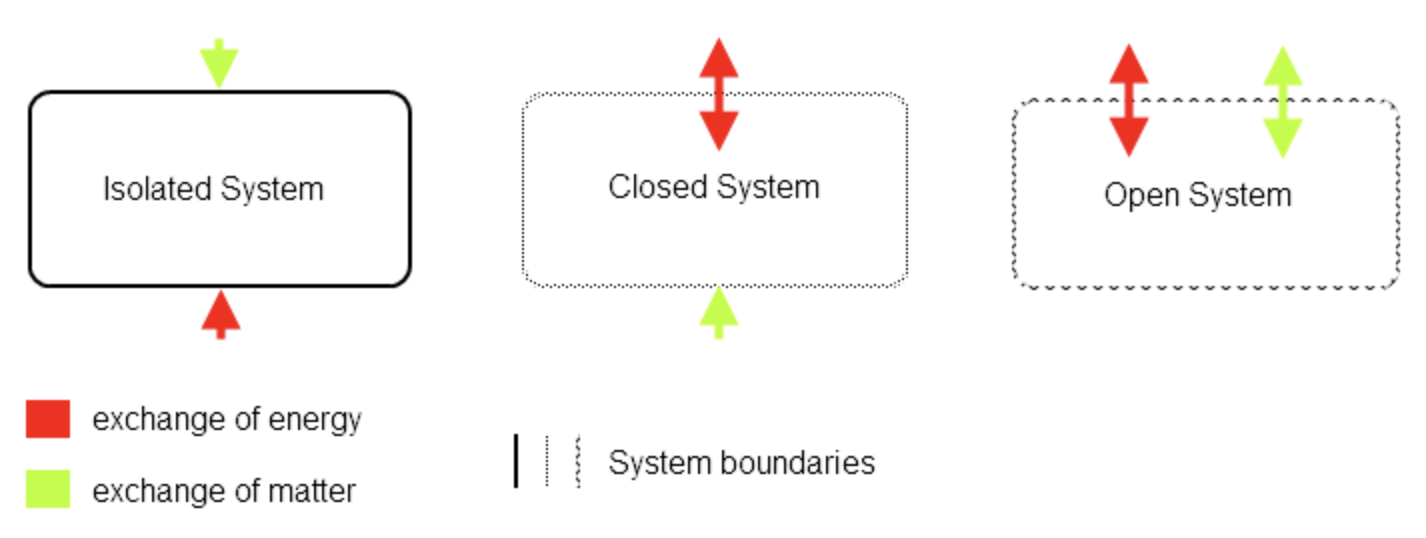
\includegraphics[scale=0.5]{systems}
	\caption{Types of systems, illustrated}
\end{figure}

\subsection*{The four laws of thermodynamics}
Only four laws are required to construct the relationships that control much of classical thermodynamics. Theses are, in brief:
\begin{itemize}
\item {\bf Zeroth law} Defines temperature and thermal equilibrium. 
\item {\bf First law} Formulates the principle of conservation of energy for thermodynamic systems, heat/work are forms of energy; energy is conserved.
\item {\bf Second law} Entropy increases and systems involve towards equilibrium; heat spontaneously flows from high to low temperatures.
\item {\bf Third law} The absolute zero of temperature is not attainable and entropy $\rightarrow$ constant as $T \rightarrow 0$.
\end{itemize}


We'll look the first two laws in a bit more detail and then make use of the second law to derive some familiar properties of heat.

\subsection{The zeroth law:}
If two systems are each in thermal equilibrium with a third system, then they are also in thermal equilibrium with each other. This implies that they have some property in common. We call this property \emph{temperature}. (In the language of mathematics we would say that thermal equilibrium is a transitive property.)

It is worth noting that thermal equilibrium is not the same as thermodynamic equilibrium. For the latter we also need mechanical equilibrium ($p_1=p_2$ --- there are no unbalanced forces) and chemical equilibrium ($\mu_1=\mu_2$ --- equal rates of reaction).

\subsection{The first law}
Heat and work are both forms of energy. The first law of thermodynamics says that energy remains constant for a (collection of) system(s) isolated from their surroundings. We denote work done \emph{on} the system by the surroundings as $W>0$, similarly, heat supplied to the system is denoted $Q>0$. The opposite sign convention holds when it is by the system. Work is path dependent, i.e. it does not only depend on the initial and final states of the system.

When considering the change in energy $\Delta E$ of a system it is necessary to consider both work and heat. For example, if system $A$ gains energy from system $B$, $\Delta E_A = -\Delta E_B \implies \Delta E_A + \Delta E_B =0$. Since, in general, $\Delta E_A\neq W_{B\rightarrow A}$ there will also be a heat flow $Q_{B\rightarrow A}$, due to a temperature difference between systems $A$ and $B$.
So,
$$\Delta E_A = W_{B\rightarrow A} + Q_{B\rightarrow A}$$
$$\Delta E_B = W_{A\rightarrow B} + Q_{A\rightarrow B}.$$

Energy conservation gives 
$$\underbrace{(W_{A\rightarrow B}+W_{B\rightarrow A})}_{\text{Work done by the composite system}} + \underbrace{(Q_{A\rightarrow B}+Q_{B\rightarrow A})}_{\text{Heat flow in the composite system}} = 0$$

In an isolated system the first law gives a sort of balance sheet for energy:
$W_{A\rightarrow B}+W_{B\rightarrow A} = 0$ and $Q_{A\rightarrow B}+Q_{B\rightarrow A}$.

% Revision: Adiabatic work and heat flow. Path dependence of work.
% You may want to incorporate the relevant content about the above concepts into this document.

Suppose work $dW = -p dV$ is done on a closed system and heat is also introduced, but thermodynamic equilibrium is maintained. Then, the change in the internal energy $U$ is $\text{d}U = \text{d}W + \text{d}Q$.


If work is done adiabatically (no energy or matter transfer), then entropy $S$ is constant, so $\text{d}Q = T \text{d}S = 0$. Therefore, $\text{d}U = \text{d}W = -p \text{d}V$.


\textit{When N is constant:} If heat is introduced with no change in volume or other such variable, $\text{d}W = 0$ so $\text{d}U = \text{d}Q = T \text{d}S$.


\textit{When N is not constant:} If heat is introduced with no change in volume or other such variable, $\text{d}W = 0$ so $\text{d}U = \text{d}Q = \mu \text{d}N$.

\subsection{The second law}
The approach to equilibrium has to be characterized by an entropy that increases steadily up to the asymptotic value corresponding to equilibrium. This defines an \textit{irreversible process}.


In a \textit{reversible} process with $\text{d}W = 0$ the entropy necessarily remains fixed at whatever maximal value it had.


Heat flows from hot to cold. Systems in thermal contact will experience this until the temperatures are equal.


If particles can flow from one system to another, they do so with chemical potential from high to low until equal.

\subsection{Internal energy}
The \emph{internal energy} of a system is the energy associated with the internal degrees of freedom of the system. This includes energy that might come from the motion of particles within the system, along with energy due to internal degrees of freedom that might be associated with the molecules that comprise those particles, for example rotational and vibrational degrees of freedom. 

The equation of state for internal energy is often written as $E = E(S,V,N)$ where $S$ is entropy, $V$ is the volume of the system and $N$ is the number of particles. (Note - all of these are extensive variables.)
Looking at the first of these, we can calculate the total derivative of the $E$. We get
$$
	\mathrm{d}E = \frac{\partial E}{\partial S}\mathrm{d}S +  \frac{\partial E}{\partial V}\mathrm{d}V +  \frac{\partial E}{\partial N}\mathrm{d}N.  
$$

The partial derivatives above must be physically relevant. We identify these as 
$$
T =  \frac{\partial E}{\partial S}, \quad p = -\frac{\partial E}{\partial V},\quad \mbox{and}  \quad \mu = \frac{\partial E}{\partial N};
$$ 
temperature, pressure and chemical potential, respectively. (Note the sign on the term for pressure.) This also suggests that we could write the equation of state for internal energy using the intensive variables that we found as the dual variables of $S$ and $V$; namely $E = E(T,p,N)$.

\subsection{Intensive and extensive variables}

\emph{Intensive} variables control the state of a system but are independent of the system size. For example: temperature $T$, pressure $p$, density $\rho$, chemical potential $\mu$

\emph{Extensive}, or additive, variables are proportionate to the size of a system (i.e. they depend on $N$). For example: energy $E$, entropy $S$, heat capacity $C$, particle number $N$, volume $V$.
One important extensive variable is the entropy (or disorder) of a system. As we just showed above, entropy is related to temperature by the internal energy $E$.

It is often helpful to think of intensive and extensive variables as coming in dual pairs with the intensive variable being the derivative of the internal energy with respect to the corresponding extensive variable given all other extensive variables are held constant. For example, $T = \frac{\partial E}{\partial S}\vert_{V,N}$.

Given two systems 1 and 2, an extensive variable for the composite system $1\cup2$ can be found by simply adding the individual extensive variables. For example, $N_{1\cup2} = N_1 + N_2$, $V_{1\cup2} = V_1 + V_2$, $E_{1\cup2} = E_1 + E_2$ ($E$ = internal energy). But this assumption clearly depends on the structural details of the interface. Imagine the oil-water interface in an emulsion like mayonnaise --- in this case the ratio  $\frac{E_{int}}{E_1+E_2}$ is more like $\mathcal{O}(1)$.
Similarly, if there are significant long range interactions, it may not be true that we can treat the extensive variables as being truly additive.
\begin{figure}[H]
	\begin{center}
		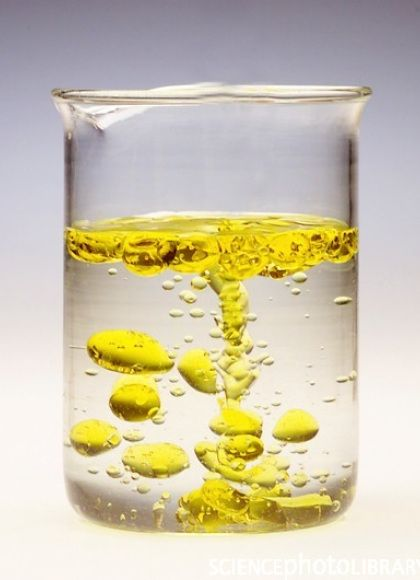
\includegraphics[width=0.2\textwidth]{oilwater}
	\end{center}
	\caption{Oil-water interface}
\end{figure}
The internal energy is not entirely an extensive variable. Since there is often an interaction term between the two systems at the interface. i.e. $E_{1\cup2} = E_1+E_2+E_{int}$. Since $E_{int}$ depends on the interface between the two systems it scales like an area as a function of system size, while $E_1$ and $E_2$ will scale like a volume, so typically $\frac{E_{int}}{E_1+E_2}\rightarrow0$ as the system size gets big. For example, an oil water interface.

\subsection{Heat capacity:}
Heat flowing into a system causes a change in temperature (except in the case of phase transitions). The amount of change in temperature for a given about of heat is the \emph{heat capacity} of the system. The heat capacity of a system depends, in part on the experimental conditions of the system under consideration. Two important cases are constant volume and constant pressure.

For constant volume we have
$$C_V = \frac{\delta Q}{dT}\bigg\vert_V$$
and similarly, for constant pressure,
$$C_p = \frac{\delta Q}{dT}\bigg\vert_p.$$

The first law of thermodynamics (conservation of energy) implies that $\delta Q = dE - \delta W = dE + pdV$  (since $W = Fdx$ and $F=p\times Area \implies W = pdV$). So, since $dV=0$ for constant volume,
$$
	C_V = \frac{\delta Q}{\partial T}\bigg\vert_{V} = \frac{\partial E}{\partial T}\bigg\vert_{V}.
$$


In the constant pressure case 
$$
	C_p = \frac{\delta Q}{dT}\vert_{p} = \frac{\partial E}{\partial T}\vert_{p} + p\frac{\partial V}{\partial T}\vert_{p}.
$$

If we have constant pressure with a change in heat, it implies that there is a change in volume. We define the \emph{volumetric thermal expansivity} as $\alpha_p = \frac{1}{V}\frac{\partial V}{\partial T}\vert_{p}$ and hence $V\alpha_p =\frac{\partial V}{\partial T}\vert_{p}$.

We can now write $C_p = \frac{\partial E}{\partial T}\vert_{p} + \alpha_p pV$. 


We can also find an expression for $C_p$ without resorting to introducing thermal expansivity. Constant pressure implies that $\mathrm{d}(pV)=p\mathrm{d}V$ so that $\delta Q = dE - dW = dE +pdV = d(E+pV)$. We define the composite quantity $E+pV$ as \emph{enthalpy}, $H$.

The infinitesimal for enthalpy is $dH = \underbrace{dE +pdV}_{\delta Q}+ Vdp = \delta Q + Vdp\vert_{p}$. In the constant pressure case, the last term is zero, so we get 
$$
	C_p = \frac{\delta Q}{\partial T}\bigg\vert_{p} = \frac{\partial H}{\partial T}\bigg\vert_{p}. 
$$

% This would be a good place to recall some of the other important thermodynamic quantities and to list the ones that have already been introduced.
% E.g. Entropy, enthalpy, Gibbs/Helmholtz free energy, and some important relationships that can be derived from each of the (the various partial derivatives)

\subsection{Important thermodynamic quantities}

\textit{Entropy} is discussed in section 1.10.


\textit{Enthalpy} $H$ governs the equilibrium of adiabatic processes that occur while pressure is
constant. Among all states that have the same entropy and pressure values, the state of equilibrium is the one that corresponds to the minimum value of enthalpy. Enthalpy is important for chemical reactions in open systems. If a system relaxes toward equilibrium while the pressure is kept constant, the maximum heat that can be produced by the system is equal to its variation in enthalpy. For this reason, enthalpy it is also called free heat.
\begin{align*}
	H(S, p, ..., X_{r}) &= E + pV
\end{align*}

Among all states that have the same temperature and pressure values, the state of equilibrium is that in which the \textit{Gibbs free energy} $G$ assumes the minimum value.
\begin{align*}
	G(T, p, ..., X_{r})  &= E - TS + pV
\end{align*}

The value of the \textit{Helmholtz free energy} $F$ is minimal for the equilibrium state among all virtual states at the given temperature T.
\begin{align*}
	F(T, X) &= E(S(T, X), X) - TS(T, X)
\end{align*}


\subsection{The fundamental hypothesis of thermodynamics}
It is possible to characterise the state of a thermodynamic system by specifying the values of a set of extensive variables.

\subsection{The central problem of thermodynamics}
Given the initial state of equilibrium for several thermodynamic systems that are allowed to interact, we want to be able to determine the final thermodynamic state of equilibrium. The boundaries of the systems --- adiabatic, closed, open --- determine the types of interactions that are allowed, while the four laws of thermodynamics (and the first and second law in particular) determine how the composite system evolves. We want to be able to describe a final thermodynamic equilibrium state from amongst the space of all possible states for the composite system.

Entropy plays a special role in this problem due to the entropy postulate --- the second law of thermodynamics.

\subsubsection*{The entropy postulate}
There exists a function $S$ of the extensive variables $X_1,X_2,\ldots,X_r$, called the entropy, that assumes a maximum value for a state of equilibrium among the space of possible states.

Entropy has the following properties:
\begin{enumerate}
\item Extensivity: If 1 and 2 are thermodynamic systems then $S_{1\cup2}=S_1+S_2$.

\item Convexity: If $X^1=(X_0^1,X_1^1,\ldots,X_r^1)$ and  $X^2=(X_0^2,X_1^2,\ldots,X_r^2)$ are two thermodynamic states of the same system then for $0\leq\alpha\leq1$
$$
	S((1-\alpha)X^1+\alpha X^2)\geq (1-\alpha)S(X^1)+\alpha S(X^2). 
$$
That is, the entropy of a linear combination of states for a single system is greater than or equal to the same linear combination of entropies of the individual states.
A consequence of this is that if we take derivatives with respect to $\alpha$  and then evaluate at $\alpha=0$ we get
$$
	\mbox{LHS:} \quad\frac{\partial}{\partial \alpha} S((1-\alpha)X^1+\alpha X^2) = \sum_{i=0}^r\frac{\partial S}{\partial X_i}(X_i^2-X_i^1)
$$
and
$$
	\mbox{RHS:} \quad\frac{\partial}{\partial \alpha} \left[ (1-\alpha)S(X^1)+\alpha S(X^2) \right] = S(X^2)-S(X^1).
$$

$$ \mbox{Hence,}~~ \sum_{i=0}^r\frac{\partial S}{\partial X_i}(X_i^2-X_i^1)\geq  S(X^2)-S(X^1).$$
Mathematically, this means that the entropy surface (as a function of the other extensive variables) is always below the tangent plane of a point on the surface.

\item Monotonicity: $S(E,X_1,\ldots,X_r)$ is a monotonically increasing function of the internal energy $E$. That is, $\frac{\partial S}{\partial E}\vert_{X_1,\ldots,X_r} = \frac{1}{T}>0$.
\end{enumerate}

Using these three properties, it is possible to find the final equilibrium thermodynamic state amongst the space of possible states of a system. The equilibrium state is the state with maximum entropy that satisfies the constraints on the system.

An example: Consider two closed systems, 1 and 2, in thermal contact such that they can exchange energy, but nothing else (i.e. no other extensive quantities change). The space of possible states is defined by 
$$E^1+E^2 = X_0^1+X_0^2 = E = \text{const.}$$
$$X_i^1 = \text{const.}\quad i=1,2,\ldots,r$$
$$X_i^2 = \text{const.}\quad i=1,2,\ldots,r.$$
We want to find the maximum of $S$ as a function of $E^1$ (we could just as well use $E^2$). Start by taking the derivative of $S$.

\begin{eqnarray*}
	\frac{\partial S}{\partial E^1} &=& \frac{\partial}{\partial E^1}\left(S^1(E^1,X_1^1,X_2^1,\ldots,X_r^1) + S^2(\underbrace{E-E^1}_{E=E^1+E^2},X_1^2,X_2^2,\ldots,X_r^2) \right)\\
	 &=& \frac{\partial S^1}{\partial E^1}\bigg\vert_{E^1} -  \frac{\partial S^2}{\partial E^2}\bigg\vert_{E^2=E-E^1}.
\end{eqnarray*}

For $E^1$ at equilibrium we will write $E^1_{eq}$ (sim. for $E^2$). Then to maximise $S$ we must have
$$
	\frac{\partial S}{\partial E^1}\bigg\vert_{E^1_{eq}} = \frac{\partial S^1}{\partial E^1}\bigg\vert_{E^1_{eq}} - \frac{\partial S^2}{\partial E^2}\bigg\vert_{E-E^1_{eq}}=0
$$
hence
$$
	\frac{\partial S^1}{\partial E^1}\vert_{E^1_{eq}} = \frac{\partial S^2}{\partial E^2}\vert_{E_{eq}^2}.
$$ We already have our first result --- the equilibrium state of the composite system is the one where the change in entropy of the two systems, with respect to, $E$ is equal. Since $\frac{\partial E}{\partial S} = \frac{1}{T}$ (by monotonicity) this means that the equilibrium occurs when the temperatures of the two sub-systems are equal.

Where does the heat flow to in the system in order to reach this equilibrium? The system started in an initial state with $E = E^1_{in}+E^2_{in}$. Since entropy increases to reach the maximum value at equilibrium we have 
$$
	S^1(E^1_{eq}) + S^2(E^2_{eq}) \geq S^1(E^1_{in}) + S^2(E^2_{in}),
$$ 
so,
$$ 
	S^1(E^1_{in}) - S^1(E^1_{eq})  +  S^2(E^2_{in}) - S^2(E^2_{eq})\geq 0.
$$

The convexity property of entropy means that both systems  1 and 2 have 
$$
	\frac{\partial S}{\partial E}\vert_{E_{in}}(E_{eq}-E_{in})\geq S(E_{eq})-S(E_{in})
$$ 
and from the previous expression, the RHS of this inequality is bounded below by zero so we have
$$
	\frac{\partial S^1}{\partial E^1}\bigg\vert_{E^1_{in}}(E_{eq}^1-E_{in}^1) + \frac{\partial S^2}{\partial E^2}\bigg\vert_{E^2_{in}}(\underbrace{E-E_{eq}^1}_{=E^2_{eq}}-E_{in}^2)\geq0
$$

But $E$ is conserved so $E=E^1_{in}+E^2_{in}$ and hence $E-E^1_{eq}-E^2_{in} = -(E^1_{eq}-E^1_{in})$. Therefore
$$
	\left[\frac{\partial S^1}{\partial E^1}\bigg\vert_{E^1_{in}} - \frac{\partial S^2}{\partial E^2}\bigg\vert_{E^2_{in}}\right]\left(E^1_{eq}-E^1_{in}\right)\geq 0.
$$

This implies that energy flows to the  system with higher $\frac{\partial S}{\partial E}$ and since $\frac{\partial S}{\partial E}= \frac{1}{T}$ this means that energy flows into the system with lowest temperature, until the temperatures are equal.

\subsection{Recommended reading}
\begin{itemize}
	\item Sections 2.1 - 2.10 of \emph{Statistical Mechanics in a Nutshell}
\end{itemize}


\section{Probability}
This section gives an introduction to some tools and ideas from probability theory. One of the main reasons for including it is that it lets us give background to the final sub-section on Brownian motion, but we'll also use some of the methods from here in the final section of the course on complex networks.

Physical variables can be either continuous or discrete. Continuous variables, like the spatial position of a particle ${\bf r} = (x,y,z);$ $x\rightarrow x+dx$ allow us to apply tools from differential calculus. Discrete variables (like the spin of an electron, the face of a playing card, or the energy level of a quantum particle) require a different approach. As the number of discrete states gets gets large, it is possible to approximate a discrete system by a continuous one. However, there are often statistical reasons why this is not always the best approach. (For one example of why it is not always good to approximate a discrete distribution with a continuous one, see the article ``Power-Law Distributions in Empirical Data'' by Clauset, Shalizi, and Newman, SIAM Review (2009) doi:10.1137/070710111) 

Here we are going to look at some simple discrete distributions, including one of the simplest --- the binomial distribution which describes the probability of events that can take one of only two possible outcomes. The tool we will employ to study these distributions is \emph{probability generating functions} (PGFs) (or generating functions for short). Although PGFs can be somewhat cumbersome, they provide a powerful general tool that can applied to a wide range of situations involving discrete probabilities. In this sense they are like the Taylor series of discrete probability.

\subsection{Probability generating functions}
A probability generating function (PGF) is a polynomial whose coefficients are the probabilities associated with each outcome of some random process.
For example, the PGF for an equal probability die is 
$$\calG(x) = 0x^0+\frac16x^1+\frac16x^2+\frac16x^3+\frac16x^4+\frac16x^5+\frac16x^6.$$
As an example of how PGFs are a handy general tool, say we now wanted to find the PGF for the sum when we roll two such dice. We can just multiply the PGFs to get $\calG'(x) = \calG(x)\calG(x) = 0x^0 + 0x^1+\frac{1}{36}x^1x^1+\frac{2}{36}x^1x^2+\cdots+\frac{1}{36}x^6x^6.$

More generally, the set of probabilities associated with any discrete distribution can be used as coefficients of $\calG(x)$:
$$\calG(x) = P(X=r_0)x^0+P(X=r_1)x^1+\cdots = \sum_{n=0}^\infty P(X=r_n)x^n.$$

\subsection{Properties of generating functions}
\begin{eqnarray*}
	\calG(0)&=&P(X=0)\\
	\calG(1)&=&\text{sum over all probabilities}=1
\end{eqnarray*}
The two properties above are easy to see and are not unexpected. More interesting is the fact that derivatives of PGFs can be used to obtain expressions for the mean, and higher order moments, of the distribution associated with the PGF.

\begin{eqnarray*}
	\frac{d}{dx}\calG(x)=\calG'(x)&=&\sum_r rP_r x^{r-1},\qquad\text{and}\\
	\calG''(x)&=&\sum_r r(r-1)P_rx^{r-2}.
\end{eqnarray*}

If we evaluate the first derivative of the PGF at 1 we get
$$\calG'(1) = \sum_r rP_r.$$
The expected value of an arbitrary function $f(r)$ is given by $\langle f(r)\rangle = \sum_r f(r) P(X=r)$, therefore $\calG'(1) = \langle r\rangle$ --- the expected value, or mean, of the distribution.

Similarly,  Evaluating $\calG''(x)$ at 1 gives 
$$\calG''(1) = \sum_r r(r-1)P(X=r) = \langle X(X-1)\rangle.$$

Why would we care about being able to find $\langle X(X-1)\rangle = \langle X^2 -X\rangle$? Because the variance of X, is given by 
$$ V(X) = \langle X^2\rangle -\langle X\rangle^2.$$ We are therefore able to construct $V(X)$ from combinations of $\calG$, $\calG'$, and $\calG''$.
We can use the fact that $\langle X^2 -X\rangle =\langle X^2\rangle-\langle X\rangle$ I.e. $\sum(r^2-r)P(X=r)=\sum r^2P(X=r)-\sum rP(X=r)$ to get

\begin{eqnarray}
V(X)&=&\langle X^2\rangle - \langle X\rangle^2\\
&=&\underbrace{\langle X^2\rangle -  \langle X \rangle}_{\calG''(1)} + \underbrace{\langle X\rangle}_{\calG'(1)} - \underbrace{\langle X \rangle^2}_{\calG'(1)^2}\\
&=& \calG''(1) +\calG'(1)-\calG'(1)^2 \label{eq:binvar}
\end{eqnarray}

Generating functions may not always be the shortest way to find the properties of some distribution, but they are a powerful way.

\subsection{The binomial distribution}
The binomial distribution describes the probability of getting $r$ identical outcomes from a sequence of $N$ events where each event has only two possible states, e.g. number of heads from a sequence of coin tosses, number of Au atoms from deposition of Au and Ag atoms in some sputtering process, or number of spin up electrons in an uncorrelated system.

The probabilities for the binomial distribution are given by
$$P(X=r) = \binom{N}{r}p^rq^{N-r}, ~\text{ where } \binom{N}{r} = \frac{N!}{r!(N-r)!}, ~~r=0,1,\ldots,N$$
and where (mostly) $p+q=1$.
The PGF for the binomial distribution is therefore given by $\calG(x) = \sum_{r=0}^N\binom{N}{r}p^rq^{N-r}x^r$. 
The coefficients in the binomial distribution are (not surprisingly) the coefficients from the  binomial expansion theorem. This means that instead of writing the PGF as a sum, we can easily express it (and its derivatives) as a polynomial:
\begin{eqnarray*}
	\calG(x)  &=& (xp +q)^N \\
	\calG'(x) &=& N(xp+q)^{N-1}p\\
	\calG''(x) &=& N(N-1)(xp+q)^{N-2}p^2. 
\end{eqnarray*}

Evaluating the above at $x=1$ gives:
	\begin{eqnarray*}
	\calG(1) &=& (p+x)^N = 1 ~\text{ if } p+q=\\
	\calG'(1) &=& N(p+q)^{N-1}P = Np  ~\text{ if } p+q=1\\
	\calG''(1) &=& N(N-1)(p+q)^{N-2}p^2 \\
		&=&N(N-1)p^2  ~\text{ if } p+q=1.
\end{eqnarray*}
As expected, we have $\langle X\rangle =Np$ for the event associated with the probability $p$.
Similarly, we can calculate the variance of the binomial distribution using equation \ref{eq:binvar}
\begin{eqnarray*}
	V(X) &=&\calG''(1) - \calG'(1) -\calG'(1)^2\\
		&=& N^2p^2-Np^2+Np-N^2p^2\\
		&=& N(p-p^2)\\
		&=& Np(1-p)= Npq.
\end{eqnarray*}

If you are feeling enthusiastic, compare the calculation above with the usual method for finding the variation of the binomial distribution without using a PGF.

\subsection{The expected long-run outcome of a binary process}
What is the net outcome we can expect from a sequence of $N$ binary events? What is the variance in this net outcome? How long can we expect the net outcome to remain positive? 

Think of a sequence of coin tosses where heads implies $+1$ and tails implies $-1$. We will denote the number of heads from $N$ events as $n_h$ and the number of tails as $n_t = N-n_h$, then the net outcome is $d = n_t-n_h = N-2n_h$. 

If $p=q=\frac12$ then the expected value of $d$ is $\langle d\rangle= 0$. (It's easy to check this: $\langle d\rangle = \langle N-2n\rangle = N-2\langle n\rangle = N-\frac{2}{2}N=0.$)

We want to find the variation in $d$, or rather, the root-mean-squared (rms) deviation 
$$d_{rms} = \left(\langle d^2\rangle - \langle d\rangle^2\right)^{\frac12} =  \langle d^2\rangle^{\frac12}.$$

At this point we'll drop the subscript in $n$ since we only have $n_h$ and since the probabilities are equal. From $d=N-2n$ we have $$ \langle d^2\rangle = \langle (N-2n)^2\rangle = \langle N^2 -4Nn+4n^2\rangle.$$
We know that $\langle n\rangle = \calG'(1)=Np=N/2$ and from the expressions for $\calG''(1)$ and $\calG'(1)$ we get $\langle n^2 \rangle = \calG''(1) + \calG'(1)$ where $\calG''(1) = N^2p^2 = N^2/4-N/4$. We can now calculate $\langle d^2 \rangle$.

\begin{eqnarray*}
	\langle d^2 \rangle &=& N^2 -4N\frac{N}{2}+4\left(\frac{N^2}{4}-\frac{N}{4}+\frac{N}{2}\right)\\
		&=& N^2-2N^2+N^2+N\\
		&=& N.
\end{eqnarray*}
So, $d_{rms}=\sqrt{N}$ and the variance in the net expected outcome scales like $\sqrt{N}$ as $N$ increases. I.e. after $N$ steps we expect to be a rms distance of $\pm \sqrt{N}$ away from the mean of zero.

%[You may want to add a figure of this, with N as the independent variable.]

We can now look at how this would change if the binary process had some small bias $\alpha = |p-q| >0$. In this case, at each step, the expected outcome is $\alpha$ and the bounds for the rms distance from the mean are $\alpha N\pm\sqrt{N}$. 

%[You might want to add a figure for this too.]

\subsection{Brownian motion}
Brownian motion is a model that describes the behaviour of particles in suspension (e.g. of dust in air, fine silt in dirty water) that have some velocity but which are constantly changing direction as they are buffeted by other particles. Their motion can be understood through a calculation similar to that for the net outcome of the binary process above, but in 3D.

The conceptual model that is often used when discussing Brownian motion is that of a \emph{random walk}. Consider a random walker who after $n$ steps is at the position ${\bf r} = (x,y,z)$. Each step is given by ${\bf s}_{n+1} = {\bf r}_{n+1}- {\bf r}_n$ and has step length $s_n$ in a random and uncorrelated direction ${\bf\hat{s}}_n$. Again (by symmetry) $\langle {\bf s}\rangle =0$. We want to find how far a particle might have gone after $N$ steps. We will define $\lambda^2= \langle {\bf s}^2\rangle$ --- the average square step-length. We write ${\bf r}_N$ for the position of the walker (or the particle) after $N$ steps, then
\begin{eqnarray*}
	\langle {\bf r}_N^2 \rangle &=& \bigg\langle \left(\sum_{n=1}^N{\bf s}_n\right)^2 \bigg\rangle\\
		&=& \bigg\langle \sum_{n=1}^N{\bf s}_n^2 +2\sum_{n=1}^{N-1}\sum_{m=n+1}^N{\bf s}_n\cdot{\bf s}_m \bigg\rangle\\
		&=& \sum\underbrace{\langle {\bf s}_n\rangle}_{=\lambda^2} + 2\sum\sum \underbrace{\langle {\bf s}_n \cdot {\bf s}_m \rangle}_{=\langle {\bf s}_n\rangle \cdot \langle{\bf s}_m \rangle=0}
\end{eqnarray*}

The first term in the expression is the mean squared step-length while the second term is zero since there is no correlation between the directions of each of the steps. Hence $\langle {\bf r}_N\rangle = N\lambda^2$ and the rms displacement is $\sqrt{N}\lambda$. If the number of steps is proportionate to the length of time that the particles move for, then we have that the mean-square displacement scales like $\sqrt{t}$. This is one of the key features of diffusive processes. 





\section{Statistical postulates}
So far we have looked at the macroscopic properties of a thermodynamical system and at some ways of calculating properties of random processes that obey some given probability distribution. Now it is time to combine these ideas and have a first attempt at linking the microscopic behaviour of a thermodynamic system (an idealised gas) with some of its macroscopic properties.

The behaviour of a given (mechanical) system depends on both the structure of the system --- described by its equations of motion --- and on the \emph{initial conditions} of the system. Therefore, in order to describe the behaviour of the system, we need both the laws of mechanics for the system along with some statistical postulates about the initial conditions of the system. (We could also require that we know the exact initial conditions for all the particles in the system, but this is not realistic for $\mathcal{O}(10^{23})$ particles.) Different choices of the statistical postulates can lead to different behaviour (not just different states) of the system. We will look at Maxwell's postulates for the initial positions and velocities of a dilute collection of gas particles. We will see that they allow us to derive the ideal gas law from a microscopic basis.

\subsection{An ideal gas}
We want to keep the equations of motion for our system of particles as simple as possible. We are going to assume   that our system has the following properties:
\begin{itemize}
\item We have $N$ identical  point particles, each with mass $m$, constrained in a volume $V$.
\item There are no mutual interactions --- no van der Waals effects or inter-particle forces for us!
\item The walls of the container constraining the particles are perfectly reflecting.
\item The mechanical state of the system is known when the position $\bf r$ and velocity $\bf v$ is known for each particle and these variables evolve according to Newton's laws of motion.
\end{itemize}

\subsection{Maxwell's postulates}
Maxwell's postulates translate the ideal gas assumptions from the previous section into conditions that we can use with Newton's equations of motion in order to, in principle, describe everything about the behaviour of an ideal gas. From these we can infer macroscopic properties by simply integrating over the microscopic variables of the system.

We assume that the vectors describing the initial conditions of the system are randomly distributed. More specifically:
\begin{enumerate}
\item The vectors relating to each particle are independent from each other. (e.g. there is no interaction between particles when they are close.) This is generally not true for any but the most dilute systems. For such a non-interacting system, the system's state is determined when $dN=f({\bf r},{\bf v})$ is known, where $dN$ is the number of particles in a box with sides $d{\bf r}=(dx,dy,dz)$ centered on the point ${\bf r} = (x,y,z)$ and where the corresponding velocities of the particles lie within a box d${\bf v}=(dv_x,dv_y,dv_z)$ centered on ${\bf v}=(v_x,v_y,v_z)$. This relationship defines the \emph{single-particle distribution} $f({\bf r},{\bf v})$.
\item The positions ${\bf r}$ are independent of the velocities ${\bf v}$. This means we can factorise $f({\bf r},{\bf v})$ as $f({\bf r},{\bf v})$ =$f_r({\bf r})$ $f_v({\bf v})$ .
\item The density of the gas is uniform within the volume so we can write $f({\bf r}) = N/V=\rho=$ constant inside the volume (and zero outside it).
\item The velocity components are independent of each other so we can factorise $f_v$ as $f_v({\bf v})=f_x(v_x)f_y(v_y)f_z(v_z)$.
\item The distribution $f_v({\bf v})$ is isotropic in velocity space so that $f_v$ depends only on the magnitude of the velocity $|{\bf v}| = v$
\end{enumerate}

\subsection{Micro to Macro}
Using the postulates above, we can derive a macroscopic equation of state. We will prove that Maxwell's postulates will allow us to derive the equation of state for ideal gases.
\begin{figure}[H]
	\begin{center}
		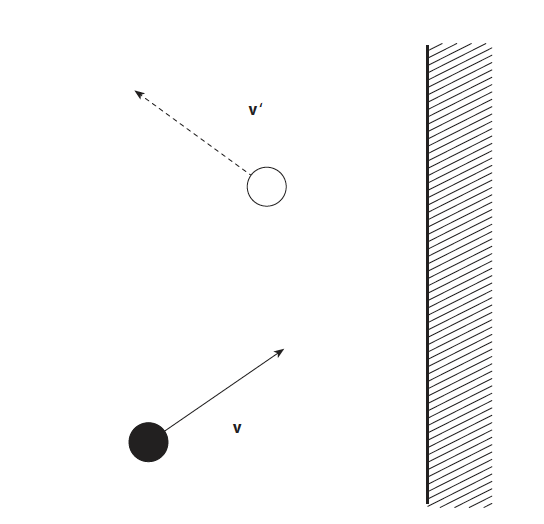
\includegraphics[width=0.4\textwidth]{bouncyboi}
	\end{center}
	\caption{Particle impacting a wall}
\end{figure}
Consider a particle with velocity ${\bf v} = (v_x,v_y,v_z)$, moving from the left, that hits a wall parallel to the $yz$-plane. After impact its velocity is ${\bf v'}=(-v_x,v_y,v_z)$. Hence, the change in momentum is $\Delta {\bf p}= {\bf p'} - {\bf p} = m({\bf v'}-{\bf v}) = m(-2v_x,0,0)$.

How many such impacts occur in a given time interval $\Delta t$ on a region of the wall with area $A$? 
Take a box with a side of area $A$ on the wall and perpendicular sides of length $v_x\Delta t$. This contains the particles of velocity ${\bf v}$ that can hit the wall. The volume of the box is $Av_x\Delta t$ and the number of particles it contains is $\rho Av_x\Delta t f_v({\bf v})$, where $\rho=N/V$ is the density of all particles  and $f_v$ is the probability that a particle has velocity $\bf v$.
The total momentum $\Delta P$ transmitted to the wall is therefore
$$\Delta P =\int_0^\infty dv_x \int_{-\infty}^\infty dv_y \int_{-\infty}^\infty dv_z f_v({\bf v})\rho A\Delta t(-2m)v_x^2{\bf i}$$
where ${\bf i} =(1,0,0)$ picks out the $x$-component. i.e. integrate over the number of particles times the momentum per particle. The first integral only runs from zero since we are only interested in particles traveling towards the right, i.e. ${\bf v}>0$. The factor of $\frac{1}{2}$ comes from integration over $v_{x}$, which runs only from $v_{x} > 0$.

The integral above gives 
$$\Delta P = -2m\rho A\Delta t \langle v_x^2\rangle\frac12$$ where the average square velocities come from integrating over the velocity distribution and the factor of half comes from the integral over $v_x$, i.e. particles moving towards the right.

The force exerted by the gas on the wall is $F=\Delta P/\Delta t$ and pressure is force/area = $|F|/A$.
We therefore have 

\begin{equation}
	p=m\rho  \langle v_x^2\rangle.
	\label{eq1.2}
\end{equation}
 
Compare this with the classical equation of state for an ideal gas $pV=NK_BT$ where $T$ is the absolute temperature and $k_B=R/N_A$ is Boltzmann's constant ($R\simeq8.3JK^{-1} \text{ mol}^{-1}$ is the ideal gas constant and $N_A\simeq6\times10^{23}mol^{-1}$ is Avogadro's number). Since $\rho = N/V$, equation \ref{eq1.2} suggests that we can relate the absolute temperature $T$ to the mean square velocities of the particles (times a constant).
\begin{align*}
	p &= \rho k_{B}T
\end{align*}



\section{Phase space, Hamiltonian dynamics, and the fundamental postulate of statistical mechanics}


\subsection{Phase space}

At a microscopic level, a thermodynamic system is comprised of $N$ particles, each with some mass $m_i$, which can interact with each other and with the boundaries of the system. (Although we are going to motivate this discussion with a thermodynamic system, everything that follows is also true for other systems where the total energy of the system is conserved --- i.e. anywhere that a Hamiltonian could show up.) If we know the positions and momenta  for each of the particles then we can completely describe the state of the system. In three dimensions, this means we must know the values for each of the $6N$ degrees of freedom (3 for position and 3 for momentum); more generally, we have $2d$ d.o.f. where $d$ is the number of d.o.f. for the positions. That is the state of the system is described by a point in a $6N$ (or $2d$) dimensional phase space.
Once a point in the microscopic phase space is know, the evolution of the system is completely governed by the equations of motion for the system. These in turn are prescribed by the Hamiltonian of the system:

$$H = T+U = H({\bf r}, {\bf v}) = H({\bf q}, {\bf p}),$$
where $T$ is the kinetic energy and  $U$ is the potential energy. In general, $H$, $T$, and $U$ may all depend on both the positions and the momenta of the particles, however, for many systems we find that, conveniently, $T = \sum_{i=1}^{N} T_i$, where $T_i=\frac{{\bf p}_i^2}{2m_i}$, and the potential $U$ depends only on the positions: $U = U({\bf q}).$

If the Hamiltonian is known for a system, then the equations of motion for that system are given by the \textit{Hamiltonian equations of motion}:
\begin{eqnarray*}
	\frac{d{\bf q}_i}{dt} &=& ~~\frac{\partial H}{\partial {\bf p_i}}, \\
	\frac{d{\bf p}_i}{dt} &=& -\frac{\partial H}{\partial {\bf q_i}}.
\end{eqnarray*}

If we write ${\bf x} = [{\bf q}^\top,{\bf p}^\top]^\top$, then we can compactly express the equations of motion as

\begin{equation}
	\frac{d{\bf x}}{dt} = f({\bf x}) = J^{-1}\nabla H({\bf x}),
\end{equation}
where
$$
	J = 
	\begin{bmatrix}
		0 & -\mathbb{I}_d\\
		\mathbb{I}_d & 0
	\end{bmatrix}.
$$
($\mathbb{I}_d$ is the identity matrix of dimension $d$.)

Given a Hamiltonian, $H$, and a suitable set of initial conditions ${\bf x}_0$, the evolution of the solution ${\bf x}(t)$ can be quite complicated (Hamiltonian systems are one of the archetypal systems for studying chaotic dynamics). However, the fact that the system is Hamiltonian provides us with some additional information that can help us characterise the state of the system. For example, it is not hard to prove that a solution ${\bf x}(t)$ that satisfies $\dot{\bf x} = f({\bf x}) = J^{-1}\nabla H({\bf x}),$ ${\bf x}_0 = {\bf x}(0)$ has $H({\bf x}(t)) = H({\bf x}_0)= const.$ That is, Hamiltonian systems conserve energy along their solutions. 

Knowing that $\frac{dH}{dt}=0$, we can reduce the size of the phase space where ${\bf x}(t)$ can lie, from $2d$ d.o.f. down to $2d-1$. If we know other quantities that remain invariant over time (e.g. the total momentum of the system) then we can further reduce the size of the phase space. Strictly speaking, there are $2d-1$ invariants (AKA first integrals or constants of motion) for a Hamiltonian system. This defines a curve in the remaining 1 d.o.f. along which the solution must lie (that is, a line in the phase space). This can be seen as a consequence of the uniqueness theorem for differential equations (think back to the 2nd year maths course on D.E.s). In reality, we typically can't find a closed form expression for most of these conserved quantities and have no idea what they might be.

It is possible that a (vanishingly) small change in the positions of the particles in phase space can lead to a large change in the state of the system and in the subsequent trajectories of the particles.
This is similar to saying that the dynamics of a Hamiltonian system can switch abruptly from regular to chaotic motion, as some parameter of the system is varied. 
Such quantities are not helpful in characterising the thermodynamics of the system.
In statistical mechanics, we are interested in the invariant quantities that only change by a little when there is a small change in the microscopic variables of the system. 
foe example ${\bf x}\rightarrow {\bf x}+\delta {\bf x} \implies H\rightarrow H+\delta H$.

One way to phrase this is to say that we want to consider systems where the region in phase space where the system is evolving can be (almost) completely identified, for thermodynamic purposes, by the values of a (not too large) number of observable invariant quantities.

\subsection{Observables}
In statistical mechanics, we say that an observable is a function defined on the phase space of the system that varies smoothly with changes in the representative point of the system. 

The kinetic energy $\sum_i \frac{p_i}{2m_i}$ is an observable, while the function $\Theta = \prod_i \theta(r_0^2-r_i^2)$, where $\theta(x)$ is the Heaviside function, is not, since an arbitrarily small change in a position $r_i$ can lead to a finite change in $\Theta$. This behaviour is not smooth which means $\Theta$ is not an observable. 

Other examples of (thermodynamic) observables include the internal energy $E$ (i.e. the Hamiltonian) and the number of particles in the system ($N = \int d{\bf r}\sum\delta({\bf r}-{\bf r}_i)$).
It turns out that the entropy $S=S(X_0=E=H,X_1,\ldots,X_r)$ is also an observable. We don't yet have a way to express the entropy as a function of the microscopic state of the system and its equations of motion. To do so, we are going to invoke the fundamental postulate of statistical mechanics.

\subsection{The fundamental postulate of statistical mechanics}
The fundamental postulate expresses the entropy $S$ as a function of the accessible volume of the phase space of a dynamical system --- that part of the phase space where the observables have values that are compatible with a specific thermodynamic state.

Assume that the thermodynamic state of a system is determined by the extensive variables $X_1,\ldots,X_r$ and that each of the $X_i$ can be expressed as a function over the microscopic phase space; I.e. $X_i = X_i({\bf x})$.
The region of phase space that is accessible is defined by the value of $X = (X_1,\ldots,X_r)$. Well, almost; we actually also allow for small discrepancies $\epsilon_i,~~i=1,\ldots,r$ to account for the effect of any non-extensive terms.

We denote the region of phase space in which the observable $X_i$ have the specific values that match the thermodynamic state as $\Gamma$ and we denote the corresponding phase space volume $\text{vol}(\Gamma)=\Omega$. Then the fundamental postulate of thermodynamics states that
\begin{equation}
	S = k_B\ln(\Omega),
	\label{eqS}
\end{equation}
where $S$ is the thermodynamic entropy, $k_B$ is Boltzmann's constant ($k_B = 1.384\times10^{-23}$J/K) and the equality should be interpreted as meaning ``is equal, up to terms of size $\epsilon_i$''. The accessible phase space volume $\Omega$ measures the amount of the phase space available to the microscopic system while it is in this macroscopic state. If the system had only discrete micro-states, then we could simply count the number of micro-states that correspond to the same macro-state. 


\subsection{Symplectic transformations and phase space area preservation}
Why is phase space so important in the formulation of entropy? To understand this we are going to look closer at some of the properties that being Hamiltonian impose on a system, including the choice of coordinate system.

We saw earlier that the equations of motion for a time-independent Hamiltonian system can be written as $\frac{d{\bf x}}{dt} = f({\bf x}) = J^{-1}\nabla H({\bf x})$. This Hamiltonian form is not preserved by arbitrary coordinate transformations;  but it \emph{is} preserved by \emph{symplectic} transformations.

{\bf Definition:} A linear transformation $A: \mathbb{R}^{2d}\rightarrow\mathbb{R}^{2d}$ is said to be symplectic if it satisfies
$$ A^\top J A = J.$$
For a non-linear transformation $\mathcal{A}$, we replace $A$ above with its Jacobian $D\mathcal{A}$.

An alternative, but equivalent, definition of a symplectic transformation --- and one that will turn out to be useful in a bit --- borrows some tools from differential geometry. (No prior experience with differential geometry is assumed.)

{\bf Definitions:} A symplectic transformation is a diffeomorphism (a smooth, invertible mapping between manifolds) $f:\mathbb{R}^{2d}\rightarrow\mathbb{R}^{2d}$, with coordinates $q$ and $p$, which preserves the symplectic two-form $\omega$ (an anti-symmetric, bilinear form) that acts on pairs of vectors and gives the sum of the oriented areas that they define. In two dimensions, this is the area of the parallelogram spanned by the two vectors.

More explicitly,
\begin{equation*}
	\omega(u,v) = u^\top Jv = \sum_{i=1}^d u_{p_i} v_{q_i} - u_{q_i} v_{p_i}.
\end{equation*}

At this point it is necessary to introduce a (potentially) new concept --- the flow map of a vector field. The flow $\varphi_{t,f}({\bf x})$ of a Hamiltonian system is a function that maps a point ${\bf x}^*$ in the phase space of the system with equations of motion $\dot{\bf x} = f({\bf x}) =J^{-1}\nabla H({\bf x})$ forward by time $t$. That is, for any $f({\bf x})$ and ${\bf x}_0$, $\varphi_{t,f}({\bf x}_0)$ gives the solution to $\dot{\bf x}=f({\bf x})$ at time $t$. 

{\bf Theorem:} If the Hamiltonian $H({\bf x})$ is a twice differentiable function on some neighbourhood of $\mathbb{R}^{2d}$, then the time-$t$ flow map $\varphi_{t,f}({\bf x}_0)$ of the Hamiltonian vector field is a symplectic map for all $t$.\\

{\bf Proof:} We will show that $\omega(u,v)=u^\top J v$ is constant along solutions of $\dot{\bf x} = J^{-1}\nabla H({\bf x})$.

The tangent vector $u(t) = \frac{\partial \varphi_t}{\partial {\bf x}_0}({\bf x}_0)u(0)$ satisfies $\frac{du}{dt} = J^{-1}\nabla^2H({\bf x}(t))u(t)$ and the tangent vector $v(t)$ satisfies a similar expression. Now we can calculate the time derivative of $\omega(u,v)$.
\begin{eqnarray*}
	\frac{d}{dt}\omega(u,v) &=& \dot{u}^{\top}Jv+u^\top J\dot{v}\\
		&=& (J^{-1}\nabla^2Hu)^\top Jv + u^\top JJ^{-1}\nabla^2Hv\\
		&=& 0
\end{eqnarray*}
since $J^{-\top}=(J^{-1})^\top$, $J^{-\top}J=-I$ and $JJ^{-1} = I$.

As the system evolves according to its equations of motion, it always preserves the area for $d=1$, or the sum of the oriented areas for $d \geq2$.


\subsection{Liouville's theorem and preservation of phase space volume}
We are now in a position to prove that the flow of a Hamiltonian system preserves phase space volume. That is, for every bounded, open set $A\subset\mathcal{R}^{2d}$ and every $t$ for which $\varphi_{t,f}({\bf x})$ exists
$$\text{Vol}(\varphi_{t,f}(\Gamma))=\text{Vol}(\Gamma)$$
where $f=J^{-1}\nabla H$ and $\text{Vol}(\Gamma) = \int_{\Gamma}d{\bf x}$.

To prove this, we will actually prove a slightly more general case: the flow of a differential equation $\dot{\bf x}=f({\bf x})$ in $\mathbb{R}^n$ is volume preserving if and only if it is divergence-free; i.e. $\nabla\cdot f=0$.

But first, why do we care about preservation of phase space volume? The fundamental postulate of statistical mechanics, $S=k_B\ln(\Omega)$ related the entropy of a system to the volume of the part of the phase space accessible to that system when it is in that particular thermodynamic state. We would like to be sure that this quantity doesn't vary too much over time as the microscopic system evolves, according to the Hamiltonian equations of motion. Although the microscopic system might be in continuous motion, the trajectories of the particles it is comprised of are such that the extensive variables which characterise the macroscopic state of the system are (almost) constant. I.e. there is no change in entropy, no heat flow, no work done while the system is at equilibrium. This is reassuring --- it says that disorder doesn't increase unless something happens.

{\bf Proof: volume preservation:}
The Jacobian of the flow map $\varphi_{t,f}({\bf x}_0)$ defines the matrix function $X(t)=D\varphi_{t,f}({\bf x}_0)$. The volume of the shape spanned by the columns of $X$ is given by $\det(X)$, and $X(t)$ is a solution of the equation
$$
\dot{X}=A(t)X(t),\qquad X(0)=I,
$$
where $A(t):=Df({\bf x}(t))$ denotes the Jacobian of $f({\bf x}(t))$ evaluated at ${\bf x}(t)=\varphi_{t,f}({\bf x}_0)$. To show that the volume defined by $X$ is constant we use the Abel-Liouville-Jacobi-Ostrogradskii identity to find the time derivative of $\det X$:
$$
\frac{d}{dt}\det X(t)=\text{trace} A(t)\cdot\det X(t).
$$
Since $A(t)=Df({\bf x}(t))$ we have $\text{trace} A(t)=\sum_i\frac{\partial f_i}{\partial {\bf x}_i}({\bf x}(t))=\nabla\cdot f({\bf x}(t))$ and therefore $\det X(t)=\det X(0)=1$ if and only if $\nabla\cdot f({\bf x})=0.$

\subsection{Recommended reading}
This section has mostly followed the first half of chapter 3 of \emph{Statistical Mechanics in a Nutshell}. However, some of the significance of Hamiltonian systems is lost in SMiaN, so I've supplemented it with more substantive (mathematically oriented) details from \emph{Geometric Numerical Integration} by E. Hairer, Ch. Lubich and G. Wanner (Springer, 2006) --- one of the best books on (the numerics of) Hamiltonian dynamical systems and a personal favourite.

\section{Molecular dynamics and simulating Hamiltonian Systems}

Much of the point of statistical mechanics is to \emph{avoid} dealing with the dynamics of microscopic systems by studying their aggregate (or extensive) properties in a statistical fashion. Given this, and the computational challenges of dealing with the dynamics of very large numbers of (probably interacting) particles, you might think that direct simulations don't have much or a role to play in statistical mechanics. But:
\begin{itemize}
	\item It isn't always tractable (or it's just plain difficult) to find analytical expressions or sufficiently accurate approximations for all properties of interest in all stat mech systems.
	\item Computing power is increasingly cheap and the size/complexity of the systems that we can study via simulation are always improving.
	\item Simulations let us directly test assumptions about what effects are important to a system by, for example, simulating a different interaction term or different geometries.
	\item There are many simulation approaches where clever heuristics allow us to deal with much larger systems than might be expected, while still getting the physics correct. (E.g. Monte Carlo methods --- this will be covered in Elke's content in the second part of the course) In some cases physical laws, such as energy-conservation, or preservation of phase space volume can be incorporated in the simulation, such that the simulation automatically preserves the appropriate behaviour, allowing us to test assumptions with simulations while ensuring that we retain the features of the system that we already know to be important.
\end{itemize}

We're going to look in more detail at this last point --- how we might ensure that we can run a simulation that preserves physical laws. The context that we are going to look at is molecular dynamics.

As you might expect from the previous section, such systems can be described by specifying a Hamiltonian where the kinetic energy component takes the familiar form
$$ T = \sum_i \frac{{p}_i^2}{2m_i},$$
where the $p_i$ are the momenta of the molecules and $m_i$ are their masses.

Interactions between particles are described by $U$, the potential term of the Hamiltonian. About the simplest model would be to treat each particle as a hard sphere, with no interactions between them, except during collisions.
An interaction term that is only slightly more complicated, but is much more realistic, is given by the Lennard-Jones potential:
$$
	U({\bf q}) = 4\epsilon_{ij}\left(\left(\frac{\sigma_{ij}}{q_{ij}}\right)^{12} - 2\left(\frac{\sigma_{ij}}{q_{ij}}\right)^{6}\right),
$$
where $|q_{ij}| = |q_i-q_j|$ are the inter-atomic separations and the $q_i$ are the positions of the particles' centers of mass. It's not hard to see that the potential has an absolute minimum at $q = \sigma$ --- this corresponds to the equilibrium separation between atoms. (Omitting the factor of 2 in the potential means the location of the minimum picks up a factor of $2^{-6}$.) The $\epsilon_{ij}$ terms gives the depth of the potential well --- the strength of the inter-atomic attraction. 

As a brief historical aside, the $q^{-6}$ term in the potential can be derived mathematically as the attraction due to induced-dipole -- induced dipole interaction. This was known before Lennard-Jones, whose contribution was to include a term for the repulsion when the inter-atomic distance gets very small (Pauli repulsion due to overlapping wave-functions for electrons that are closer than the preferred bonding distance). The repulsion term is actually exponential, not $q^{-12}$, but Lennard-Jones decided that $q^{-12}$ is pretty close to an exponential, and is much easier to calculate. Once you already know $q^{-6}$ you can just square it and save yourself a (relatively) expensive calculation of an exponential.

It is worth noting that the pairwise interactions in the Lennard-Jones potential mean that for $N$ particles we must calculate $N^2$ interaction terms. Clearly, this can cause issues once N gets large. One common approach is to use a \emph{long-range cut-off} and only calculate the interaction terms for atoms that are less than some distance $L$ away, or perhaps, only for those inside a unit cell, with sides of length $L$.

Regardless of the exact nature of the interaction term, we end up with a Hamiltonian of the form 
$$
	H({\bf q},{\bf p}) = T({\bf p}) + U({\bf q}).
$$

\subsection{Numerical integration}
Given the equations of motion that describe a Hamiltonian a system, and some compatible initial conditions ${\bf x}(0)$, we want to find the state of the system at some time $T$ in the future (or the solution along some interval $[0,T]$). We do this by breaking the interval into small enough time steps of size $h$ and discretizing the solution ${\bf x}(t)$ as ${\bf x}_n = {\bf x}(t_n) $ where $t_n = nh$.

The simplest approach to approximating the discrete solution is the \emph{explicit Euler method}. It approximates the solution at ${\bf x}(t_{n+1})\simeq {\bf x}_{n+1}$ with
$$
	{\bf x}_{n+1} = {\bf x}_n + h \dot{\bf x}_n.
$$
That is, it evaluates the differential equation at the current time step and approximates the solution with a straight line of slope $\dot{\bf x}_n$. 

[You can add a diagram to illustrate this - even a hand drawn example.]

The error in the approximation of the solution by the explicit Euler method grows in proportion to the step size $h$; that is, $\|{\bf x}_N-{\bf x}(Nh)\|=\mathcal{O}(h)$. We therefore say that the method is first order accurate.

While the explicit Euler method is very easy to implement, it has a number of issues (you'll see one of them in the assignment). These include the fact that it becomes unstable (the error in its approximation starts to grow exponentially) when the step size is too large. The \emph{implicit Euler} (like the explicit Euler method, but the derivative is evaluated at the end of the time step i.e.$f(x_{n+1})$) method avoids this issue, but at the cost of needing to iteratively solve an implicit equation $x_{n+1}=x_n+hf(x_{n+1})$. It is still only first order.

Since $M\dot{\bf q} = {\bf p}$ and $M\ddot{\bf q} = \dot{\bf p}$ the equations of motion for the system can be written as
\begin{equation}
	M\ddot{\bf q} = f({\bf q}) = -\nabla U({\bf q}).
	\label{eq:2vf}
\end{equation}
That is, we can turn the set of $2d$ first-order differential equations in ${\bf q}$ and ${\bf p}$ into $d$ second order differential equation in ${\bf q}$.
In much of what follows, I'm going to omit the mass matrix and write $\ddot{\bf q} = f({\bf q})$. This is purely for convenience. Everything still holds when $M$ takes other values for the masses --- just make sure to include a factor of $M^{-1}$ in the $f({\bf q})$ term.

A better approach to numerical integration is to use the Verlet (AKA St\"{o}rmer, AKA leap-frog) method. This is most easily understood in its \emph{two-step formulation} (i.e. the method requires information from two previously known time steps ($t_{n-1}$ and $t_n$) in order to compute the approximation at the future time step $t_{n+1}$). The approximation is given by 
\begin{equation}
	\frac{{\bf q}_{n+1} - 2{\bf q}_n + {\bf q}_{n-1}}{h^2} \simeq f({\bf q}_n) = \ddot{\bf q},
	\label{eq:2lf}
\end{equation}
where $f({\bf q})$ is the second order differential equation in equation \ref{eq:2vf}. It's not hard to see (you should verify it yourself) that the LHS of \ref{eq:2lf} is an approximation of the second derivative at the point ${\bf q}_n$.

[add a picture to illustrate this]

The two-step formulation of the leapfrog method can therefore be seen as determining a parabola that interpolates the points ${\bf q}_{n-1},~{\bf q}_{n},$ and ${\bf q}_{n+1}$ and matches the second derivative at the midpoint.

It turns out that, for a number of reasons, it is better to work with the Verlet method in its one-step formulation. This can be derived by introducing the velocity $p=\dot{\bf q}$ and turning equation \ref{eq:2vf} back into a first-order system of twice the dimension
$$
	\dot{\bf q} = {\bf p},\qquad \dot{\bf p} = f({\bf q}).
$$

We then introduce discrete approximations of $q$ and $p$ as follows:
$$
p_n =\frac{q_{n+1}-q_{n-1}}{2h},\qquad p_{n-\frac12} = \frac{q_n-q_{n-1}}{h}, \qquad q_{n-\frac12} = \frac{q_n + q_{n-1}}{2},
$$
where some of the values have been calculated on a staggered grid. We can then use these to formulate a one-step version of the Verlet method. 
\begin{eqnarray*}
	{\bf p}_{n+\frac12} &=& {\bf p}_n+\frac{h}{2}f({\bf q}_n),\\
	{\bf q}_{n+1} &=& {\bf q}_n +h{\bf p}_{n+\frac12},\\
	{\bf p}_{n+1} &=& {\bf p}_{n+\frac12}+\frac{h}{2}f({\bf q}_{n+1}).
\end{eqnarray*}

[Add a picture to illustrate this]

There is also a dual formulation of the method that gives the values of ${\bf q}$ and ${\bf p}$ on the staggered grid points $t_{n-\frac12},t_{n+\frac12},$ etc.
(It makes sense to think of the one-step method as a discrete map $\Phi_h$, similar to the flow map $\varphi_{f,t}$ that maps from the known solution, to its approximation one time step forward.)

If the velocity values are not needed at the end of each step, then the last line of one step can be combined with the first line of the next step to avoid one evaluation of $f$ per step by only calculating ${\bf p}$ on the staggered grid:
\begin{eqnarray*}
	{\bf p}_{n+\frac12} &=& {\bf p}_{n-\frac12}+hf({\bf q}_n),\\
	{\bf p}_{n+1} &=& {\bf q}_n +h{\bf p}_{n+\frac12}.
\end{eqnarray*}
This is the most computationally efficient form of the Verlet method. It is also numerically more stable than the two-step formulation.

It is not too hard to show (you should prove it for yourself) that the Verlet method is symplectic. That is, the discrete map that it defines preserves the symplectic form that we saw earlier. This is almost, but not quite the same as preserving the value of the associated Hamiltonian along solutions of the vector field. In fact, it is possible to show (but trickier than proving symplecticity) that the difference between the value of the Hamiltonian evaluated along the discrete approximation from the Verlet method differs only exponentially slowly from the exact value of the Hamiltonian for the true solution. This makes the Verlet method a popular choice for molecular dynamics. In addition to having good stability and being easy to implement, it is automatically almost energy-preserving.

The Verlet method is \emph{symmetric} (replacing $h$ with $-h$ and swapping the subscripts $n$ and $n+1$ gives the same method again) and \emph{reversible} (changing the sign on the velocity for the initial condition is the same as running the method in reverse). It is also second order accurate; that is the error in the solution $\|{\bf x}_{Nh}-{\bf x}(Nh)\|=\mathcal{O}(h^2)$.

Now that we have a suitable method for calculating the micro-state of a system at some point in the future, we can look for ways to measure macroscopic quantities from the solution. It is worth bearing in mind that for any simulations, the initial conditions used are unlikely to correspond to a representative configuration for the system. It is therefore good practise to let the simulation run for a period of time (perhaps a few thousand time steps) before attempting to measure any properties. This process is known as equilibration or thermalization.

Using simulated particle trajectories usually means we implicitly invoke an assumption of \emph{ergodicity}. This essentially says that averaging an observable along a solution, for a long enough time period for a system, is equivalent to averaging that observable over a large number of initial conditions for the same system, where the initial conditions correspond to the same macro-state of the system. While the hypothesis of ergodicity is useful, there are many real world cases where it doesn't hold --- for example any system that exhibits \emph{hysteresis} in which properties of the system are path dependent. Magnetic systems, in particular, tend to display such properties. For more discussion of this, see section 4.0 of \emph{Statistical Mechanics in a Nutshell}.

We have seen earlier that we identify the temperature of a thermodynamic system with the average square velocities of the particles in the system with some suitable normalisation. The temperature of our simulated system, with $N$ particles is therefore given by
$$
	T({\bf p}) = \frac{1}{Nk_B}\sum_{i=1}^N\frac{1}{2m_i}\|p_i\|^2.
$$

Another easily computable quantity is the virial function (we haven't mentioned this yet, but it is used to relate the total potential energy of a system to the total kinetic energy and can be used to calculate the pressure of a system --- see pp 255--256 of \emph{Statistical Mechanics in a Nutshell}):
$$
	C({\bf r}) = \sum_{i=2}^N\sum_{j=1}^{i-1}\nabla U(r_{ij})r_{ij},
$$
Both of these quantities give instantaneous values of the observables. Other quantities can be calculated as time averages of a solution of the system. For example, the constant volume specific heat:
$$
	C_v = k_B\left[\frac{2}{3N}-\frac{4}{9}\frac{\langle(T-\langle T\rangle)^2\rangle}{\langle T\rangle^2}\right]^{-1}
$$

where the angle brackets denote expected values over time.

\subsection{Recommended reading}
\begin{itemize}
	\item Sections 8.1 and 8.2 of \emph{Statistical Mechanics in a Nutshell}
	\item \emph{Geometric numerical integration illustrated by the St\"{o}rmer–Verlet method}, E. Hairer, Ch. Lubich, and G. Wanner, Acta Numerica (2003)
	\item Chapter 11 of \emph{Simulating Hamiltonian Dynamics}, B. Leimkuhler and S. Reich, Cambridge Univeristy Press (2004)
\end{itemize}


\section{Ensembles}

For a given macrostate $(N, V, E)$, a statistical system, at any time t, may be in any one of an extremely large number of distinct microstates. As time passes, the system transitions between different microstates, all of which correspond to the same macrostate, with the result that, over a long enough time period the behaviour of the systems is ``averaged'' over the collection of microstates which have been visited by the system.
A useful approach is to consider, at a single instant of time, a large (infinite) number of copies of the same system, existing in all possible microstates that satisfy the macroscopic conditions. Then, we can expect the average behaviour of any system for this collection (or ensemble) to be identical with the time-averaged behaviour of the system. This forms the basis of the so–called ensemble theory.

\subsection{The micro-canonical ensemble}
In the previous section, we considered an isolated system where we could keep track of the dynamics of every particle and use that to calculate the values of extensive, macroscopic properties of the system. An important aspect of this was the conservation of energy for the system. We refer to such systems as a \emph{micro-canonical ensemble} --- the system is isolated with no heat flux and no change in the number of particles, hence the internal energy of the system is constant and it is described entirely by the Hamiltonian dynamics.

Since $H=E=\mbox{const.}$ for a micro-canonical ensemble, we can associate the ensemble with a hypersurface $H=E$ that corresponds to a the macrostate $(N,V,E)$. However, in order to allow for small fluctuations that correspond to what is essentially the same state, (we require any observables to be smoothly varying functions of the phase space) it is often desirable to replace the hyper-surface with the hyper-shell $E-\Delta/2 \leq H \leq E+\Delta/2$. The \emph{density function} $\rho(p,q,t)$ characterises the distribution of points in phase space for a system in some state. With three d.o.f. and $N$ particles, we therefore have $\rho(p,q,t)\mathrm{d}^{3N}p\mathrm{d}^{3N}q$ as the number of representative points in phase space in a volume element $\mathrm{d}^{3N}p\mathrm{d}^{3N}q$, centred at the point $(p,q)$ at time $t$. From Liouvilles theorem, we have the $\frac{\partial \rho}{\partial t}=0$. 

When the internal energy of the system lies in $E-\Delta/2 \leq H \leq E+\Delta/2$ we have


\[ 
	\rho(p,q) = 
\begin{cases} 
      \mbox{const.} & \mbox{ if } E-\Delta/2 \leq H \leq E+\Delta/2, \\
      0 & \mbox{otherwise.} 
   \end{cases}
\]

For the hyper-shell $E-\Delta/2\leq H \leq E+\Delta/2$ the enclosed volume is
\[
\omega(E) = \int_{E-\Delta/2\leq H \leq E+\Delta/2} \mathrm{d}^{3N}p\mathrm{d}^{3N}q.
\]
We'd like to establish a numerical correspondence between $\Gamma$ and $\omega$ in order to account for the multiple microstates that can correspond to a single macrostate of the system. To do so, we introduce the concept of a \emph{fundamental volume} $\omega_0$ which we regard as being the volume equivalent to one microstate. Then $\Gamma = \omega/\omega_0$ and hence
\[
S =k \ln|\Gamma| = k\ln(\omega/\omega_0).
\]


Now, let's consider how we might work with ensembles if we have a composite system made up of two subsystems. The simplest case is two (isolated) systems in contact, without any exchange of energy. If the state of system 1 corresponds to the region of phase space $\Gamma^1$ and similarly, the state of system 2 to $\Gamma^2$ then the state of the composite system $1\cup 2$ corresponds to the phase space regions given by the Cartesian product $\Gamma^{1\cup 2}=\Gamma^1\times\Gamma^2$ and the volume of this accessible volume of phase space is given by $|\Gamma^{1\cup 2}|=|\Gamma^1||\Gamma^2|$. From this, it's easy to see that the entropy of the composite system is given by
\begin{eqnarray*}
	S &=& k_B\ln|\Gamma^{1\cup 2}| = k_B\ln(|\Gamma^1||\Gamma^2|)\\
		&=& k_B\ln|\Gamma^1| + k_B\ln|\Gamma^2| = S^1 + S^2,
\end{eqnarray*}
which is fortunate, since entropy is an extensive variable and we therefore expect it to be additive.
In this example the two sub-systems were completely isolated from each other; the dynamics of one system had no influence on the dynamics of the other. This condition of dynamic independence corresponds to the independence of the observables that pertain to these sub-systems.

Now, let's look at how the entropy of a composite system changes if we allow for the exchange of energy between the two sub-systems (a closed system). This has the effect of increasing the accessible volume of the phase space, since exchange of energy means that there are more possible configurations for the overall system.

Without energy exchange, the volume of the accessible phase space to the total system is given by
$$
	|\Gamma_0| = |\Gamma^1||\Gamma^2|.
$$
Once we allow for the exchange of energy, this becomes
$$
	|\Gamma| = \sum_{E^1}|\Gamma^1(E^1)||\Gamma^2(E_\text{tot}-E^1)|.
$$
That is, we must now consider all possible configurations where the total energy of the composite system is partitioned between the two sub-systems. This volume is bounded below by $|\Gamma_0|$ since the expression for $|\Gamma_0|$ is just one of the terms in the sum. At first glance, it may look like this increase in the volume of the accessible phase space is enormous (we have added many more possible configurations), however, the volume of the accessible phase space for the composite system corresponds almost entirely to the states where $E^1=E^1_\text{eqm}$ and $E^2=E^2_\text{eqm}$. As a consequence, for large enough $N$, the difference between $\Gamma$ and $|\Gamma^1(E^1_\text{eqm})||\Gamma^2(E^2_\text{eqm})|$ remains small. It's not too hard to show (see section 3.7 of \emph{Statistical Mechanics in a Nutshell}) that the contribution to the accessible phase space volume due to the exchange of energy between the two systems is of order $\sqrt{N}$ compared with the total system size $N$.

\subsection{The canonical ensemble}

Rather than considering a perfectly isolated system, for which energy is conserved, a more realistic experimental situation may be to consider a system S in thermal contact with some much larger reservoir R. This has the effect of holding the total system at constant temperature. In such a situation we want to be able to calculate the average value $\langle A\rangle$ of an observable $A$ for the system S; we are not interested in the state of the reservoir R, except to the extent that it helps us determine the state of S.

If, for the composite system S$\cup$R, we write $x_S,x_R$ for points in the phase space of the microscopic system, then the average value of the observable $A$ is given by
$$
	\langle A\rangle = \frac{1}{|\Gamma|}\int_{\Gamma}dx_Sdx_RA(x_s),
$$
where $\Gamma$ is the region of the phase space for the composite system, when it has total internal energy of $E$.

In order to make explicit the parts of the total phase space that is accessible to the composite system, wewrite the above expression as the Cartesian product of the phase space for the system and the reservoir, i.e.
$$
	\langle A\rangle =\frac{1}{|\Gamma|}\int dx_SA(x_S)\times\int dx_R\delta(H^R(x_R)-(E-H^S(x_S))).
$$
The delta function in the last term is zero, except when $x_S$ and $x_R$ in the two sub-systems take values such that $H^S+H^R=E$. That is the delta function defines the accessible phase space volume when the two sub-systems can exchange internal energy between them, but the total internal energy of the composite system is conserved.

Recalling the fundamental postulate of statistical mechanics ($S=k_B\ln|\Gamma|$), we rewrite the last expression to replace the phase space volume with the corresponding expression for entropy:
$$
	\int dx_R\delta(H^R(x_R)-(E-H^S(x_S))) \simeq \exp\left(\frac{1}{k_B}S^R(E-H^S)\right).
$$

Since $H^S$ is much less than $E$ it makes sense to now expand the entropy term on the right-hand side in a Taylor series about $E$:
$$
	\exp\left(\frac{1}{k_B}S^R(E-H^S)\right)\simeq \exp\left(\frac{1}{k_B}S^R(E)\right)\exp\left(\frac{-1}{k_B}\frac{\partial S^R}{\partial E}|_E H^S(x_S)\right)\ldots
$$

Earlier in the course, we associated $\frac{\partial S}{\partial E}$ with $\frac{1}{T}$; for a canonical ensemble, $T$ is constant (that's the point of the reservoir) so we write the expected value of the observable as
$$
	\langle A\rangle \simeq \frac{1}{|\Gamma|}\int dx_sA(x_S)\times\exp\left(\frac{1}{k_B}s^R(E)\right)\exp\left(\frac{-H^S(x_S)}{k_BT}\right).
$$

It remains to make the normalisation precise. When we do this, the factors of $S\exp\left(\frac{1}{k_B}S^R(E)\right)$ cancel from the integral and its normalisation and we get
\begin{equation}
	\langle A\rangle = \frac{1}{Z}\int dx_SA(x_S)\exp\left(\frac{-H^S(x_S)}{k_BT}\right),
	\label{eq:z1}
\end{equation}
where $Z$ is the known as the \emph{partition function} and is given by
\begin{equation}
	Z = \int dx_S\exp\left(\frac{-H^S(x_S)}{k_BT}\right).
	\label{eq:z2}
\end{equation}

One way to think about equations \ref{eq:z1} and \ref{eq:z2} is that we no longer need to keep track of which parts of phase space are accessible. Instead we can integrate over the entire phase space and each region is weighted appropriately, according to $\exp\frac{-H}{k_BT}$ --- the so-called \emph{Boltzmann factor}, a probability density in the phase space.

Similar to the case of the micro-canonical ensemble, for the canonical ensemble, the contributions to $A$ are dominated by the part of phase space that corresponds to when the system's internal energy is at the equilibrium value. 

You should read through, and understand, section 3.12 of \emph{Statistical Mechanics in a Nutshell} and sections 4.1--4.3 of \emph{Statistical Mechanics Made Simple} for some extra details and explanation.


\subsection{A generalised ensemble}
We can follow a similar approach to what we did for the canonical ensemble and generalise to other types of ensembles. Let's start by considering a system $S$ for which we want to specify a fixed value for $f_i$, some intensive variable, with $X_i$ as the conjugate extensive variable ($\frac{\partial S}{\partial X_i}=-\frac{f_i}{T}$). We can do this by putting the system in contact with a reservoir $R$ with which it can exchange $X_i$ such that $X_i = X_i^S+X_i^R$. Now we follow a similar procedure to that for the canonical ensemble:
\begin{eqnarray*}
	\langle A \rangle &=& \frac{1}{|\Gamma|}\int_{\Gamma}dx_R dx_S A(x_S)\\
	&=& \frac{1}{|\Gamma|}\int dx_S A(x_S)\int dx_R \delta(X_i^R(x_R)+X_i^S(x_S)-X_i)\\
	&=& \frac{1}{|\Gamma|}\int dx_S A(x_S)\exp\left( \frac{-1}{k}S(X_i-X_i^S(x_S))\right)\\
	&\simeq& \frac{1}{Z}\int dx_S A(x_S)\exp\left( \frac{-1}{k}\frac{\partial S}{\partial X_i}X_i^S(x_S)\right)\\
	&=& \frac{1}{Z}\int dx_S A(x_S)\exp\left( \frac{-1}{k} f_i X_i^S(x_S)\right),
\end{eqnarray*}
where the partition function $Z$ is given by
$$
	Z= \int dx \exp\left( \frac{f_iX_i(x)}{kT} \right).
$$
The integral in the partition function can be evaluated via the saddle point method (see the notes about this on Canvas if you want to know more) to get
\begin{equation*}
	Z \simeq \exp\left(\frac{T^S(X_i^*)+f_iX_i^*}{k_BT}\right),
\end{equation*}
where $X_i^*$ is the value of $X_i$ which maximises the value of the exponential.

(See SMiaN, section 3.13 for more on this.)

\subsection{Calculating quantities from a (generalised) ensemble}

If we want to compute the expected value of some extensive variable $X_i$ in our generalised ensemble we have
\[
	\langle X_i\rangle = \frac{1}{Z}\int dx X_i \exp\left(\frac{f_iX_i(x)}{kT}\right) = \frac{\partial \ln Z}{\partial (f_i/kT)}.
\]
Similarly,
\[
	{\partial^2 \ln Z}{\partial (f_i/kT)^2} = \langle X_i^2 \rangle - \langle X_i \rangle^2 = kT\frac{\partial \langle X_i\rangle}{\partial f_i}.
\]

As a specific example of working with the above, let's look at the expected value of the internal energy for a canonical ensemble with constant temperature. First introduce the shorthand $\beta = 1/kT$.
$$
	E = \langle H \rangle = \frac{\int E_S\exp(-\beta H_s)}{\int{\exp(-\beta H_S)}} = \frac{-\partial}{\partial \beta}\ln\int\exp(-\beta H_S).
$$

\subsubsection{Helmholtz free energy}
The \emph{Helmholtz Free Energy} is given by
$$
	F = E - TS
$$
hence
$$
	\mathrm{d}F = \mathrm{d}E - T\mathrm{d}S - S\mathrm{d}T.
$$
This gives $S= -\left(\frac{\partial F}{\partial T}\right)$ and $p = -\left(\frac{\partial F}{\partial V}\right)$. We can use this to write the  internal energy as $E=F+FS=F-T\frac{\partial F}{\partial T}=-T^2\frac{\partial}{\partial T}\left(\frac{F}{T}\right) = \frac{\partial (F/T)}{\partial (1/T)}$. So $E = \frac{\partial}{\partial \beta} F\beta$ but this is also $E = -\frac{\partial}{\partial\beta}\ln(\int\exp(-\beta H))$ so $F= \frac{-\ln(\int\exp(-\beta H))}{\beta} = -kT\ln(Z)$. From this we can calculate the specific heat $C_V = \left(\frac{\partial E}{\partial T} \right)_{N,T} = -T\left(\frac{\partial^2 F}{\partial T^2}\right)_{N,V}$.


\subsubsection{The $P-T$ ensemble}
The \emph{$p-T$ ensemble} is one specific example of a generalised ensemble. In this case the pressure and temperature are fixed, while the internal energy and volume (their conjugate variables) are allowed to fluctuate.
Using the generalised formula (see the sections above), and dropping the subscripts, the $p-T$ ensemble is given by
 \begin{equation*}
	\langle A\rangle = \frac{1}{Z}\int dxA(x)\exp\left(-\frac{E(x)+pV(x)}{k_BT}\right),
\end{equation*}
while the partition function is given by
$$
	\ln Z = -\frac{E-TS+pV}{k_BT}.
$$
The quantity on the top of the fraction is the \emph{Gibbs free energy}. (See section 3.14 of SMiaN)


\subsection{The grand-canonical ensemble}
Rather than holding $N$, the number of particles, fixed we can allow it to vary and instead specify $\mu$ the chemical potential. The corresponding ensemble for this case is the so-called \emph{grand-canonical ensemble}. Following a similar process as for the canonical emsemble we proceed by noting $N^S+N^R = N$ and $N^S<<N^R$. 

The expected value of an observable $A$ is given by
$$
	\langle A\rangle = \frac{1}{Z}\sum_{N=1}^{\infty}\int\mathrm{d}xA(x)\exp\left(-\frac{H_N(x)-\mu N}{k T}\right)
$$
and the corresponding partition function is given by
$$
	Z=\exp\left(-\frac{E-TS-\mu N}{k_B T}\right).
$$

(See section 3.15 of SMiaN and section 4.4 of SMMS for more discussion of the grand canonical ensemble.)

\subsection{Information theory and the Gibbs Formula for entropy}
To finish off this section, we'll look at one last application of entropy; not because it is particularly useful to physical systems in statistical mechanics, but because it gives a result that forms the basis of information theory.

We'll return to a considering a generalised ensemble, like the one we looked at a couple of sections earlier. However, in this case we'll assume that the phase space is discretized and that the index $n$ runs over all of the microstates of the system. If we consider an intensive variable $f$ and its corresponding extensive variable $X$ then the expression for the expected value of any observable $A$ is
$$
	\langle A \rangle = \frac{1}{Z}\sum_n A_n\exp\left(\frac{fX_n}{k_BT}\right),
$$
while the partition function $Z$ is given by
$$
	Z =\sum_n\exp\left(\frac{fX_n}{k_BT}\right).
$$

The partition function is related to the thermodynamic potentials (see the previous section on generalised ensembles and SMiaN sections 3.12 and 3.13) via
\begin{equation}
	\ln Z = \frac{TS+f\langle X\rangle}{kT}.
	\label{eq:gibbZ}
\end{equation}

Now, for any individual microstate $n$ the probability is therefore given by
$$
	p_n = \frac{1}{Z}\exp\left(\frac{fX_n}{k_BT}\right).
$$
Taking the log of both sides of this expression gives
$$
	\ln p_n = \frac{fX_n}{k_BT} - ln Z,
$$
which after substituting \ref{eq:gibbZ} for $\ln Z$ gives
$$
	\ln p_n = \frac{1}{k_BT}(fX_n -TS -f\langle X\rangle).
$$

Now we can calculate the expected value of both side of the above equation
$$
	\langle \ln p_n \rangle = \sum_n p_n\ln p_n = \frac{1}{k_BT}(f\langle X\rangle -TS -\langle X \rangle) = \frac{-S}{kB}.
$$


After rearranging this for $S$ (and making explicit the sum for the expected value of $p_n$) we arrive at the \emph{Gibbs formula for entropy}:
$$
	S = -k_B\sum_np_n\ln p_n.
$$

Although this is elegant, it's generally useless in the context of physical systems since the number of microstates it would be necessary to sum over is far to large to be computationally practical and, in any case, we generally don't know the probability distribution $p_n$ for each of the microstates. The value of this expression lies in its application to other systems, particularly information theory, where it can be used to quantify amount of information in, for example a digital signal, in which case the $p_n$ represent the probability of receiving the $n$-th possible value in the list of signals. We'll also see, later in the course that the Gibbs entropy plays a role in the statistical mechanics of complex networks.

\subsection{Recommended reading}
Most of the notes in this section follow closely the second half of chapter 3 in \emph{Statistical Mechanics in a Nutshell}; specifically, section 3.6--3.18. Chapter four of \emph{Statistical Mechanics made Simple} covers the same material in sections 4.0--4.4. It is gives some intuitive and succinct explanations, but I find it to be of more use \emph{after} you've already looked at SMiaN. Also useful, and with a slightly different presentation (perhaps with more traditional notation), is \emph{Entropy, Order Parameters, and Complexity}. Here the content is spread around a bit over chapters three through six. Much of the useful content, including some relevant to early sections of these notes, is in sections 3.1, 3.5, 6.1, 6.2, 6.3, and 5.3.


\section{Not Liouville's Theorem}
Science doesn't tell us much about whether or not Liouville liked cats but we do know that some people have used pictures of cat faces to illustrate the concept of phasespace area conservation. 
Here are a collection of cat drawings from the 742 class of 2020.


\begin{centering}
\begin{figure}\centering
	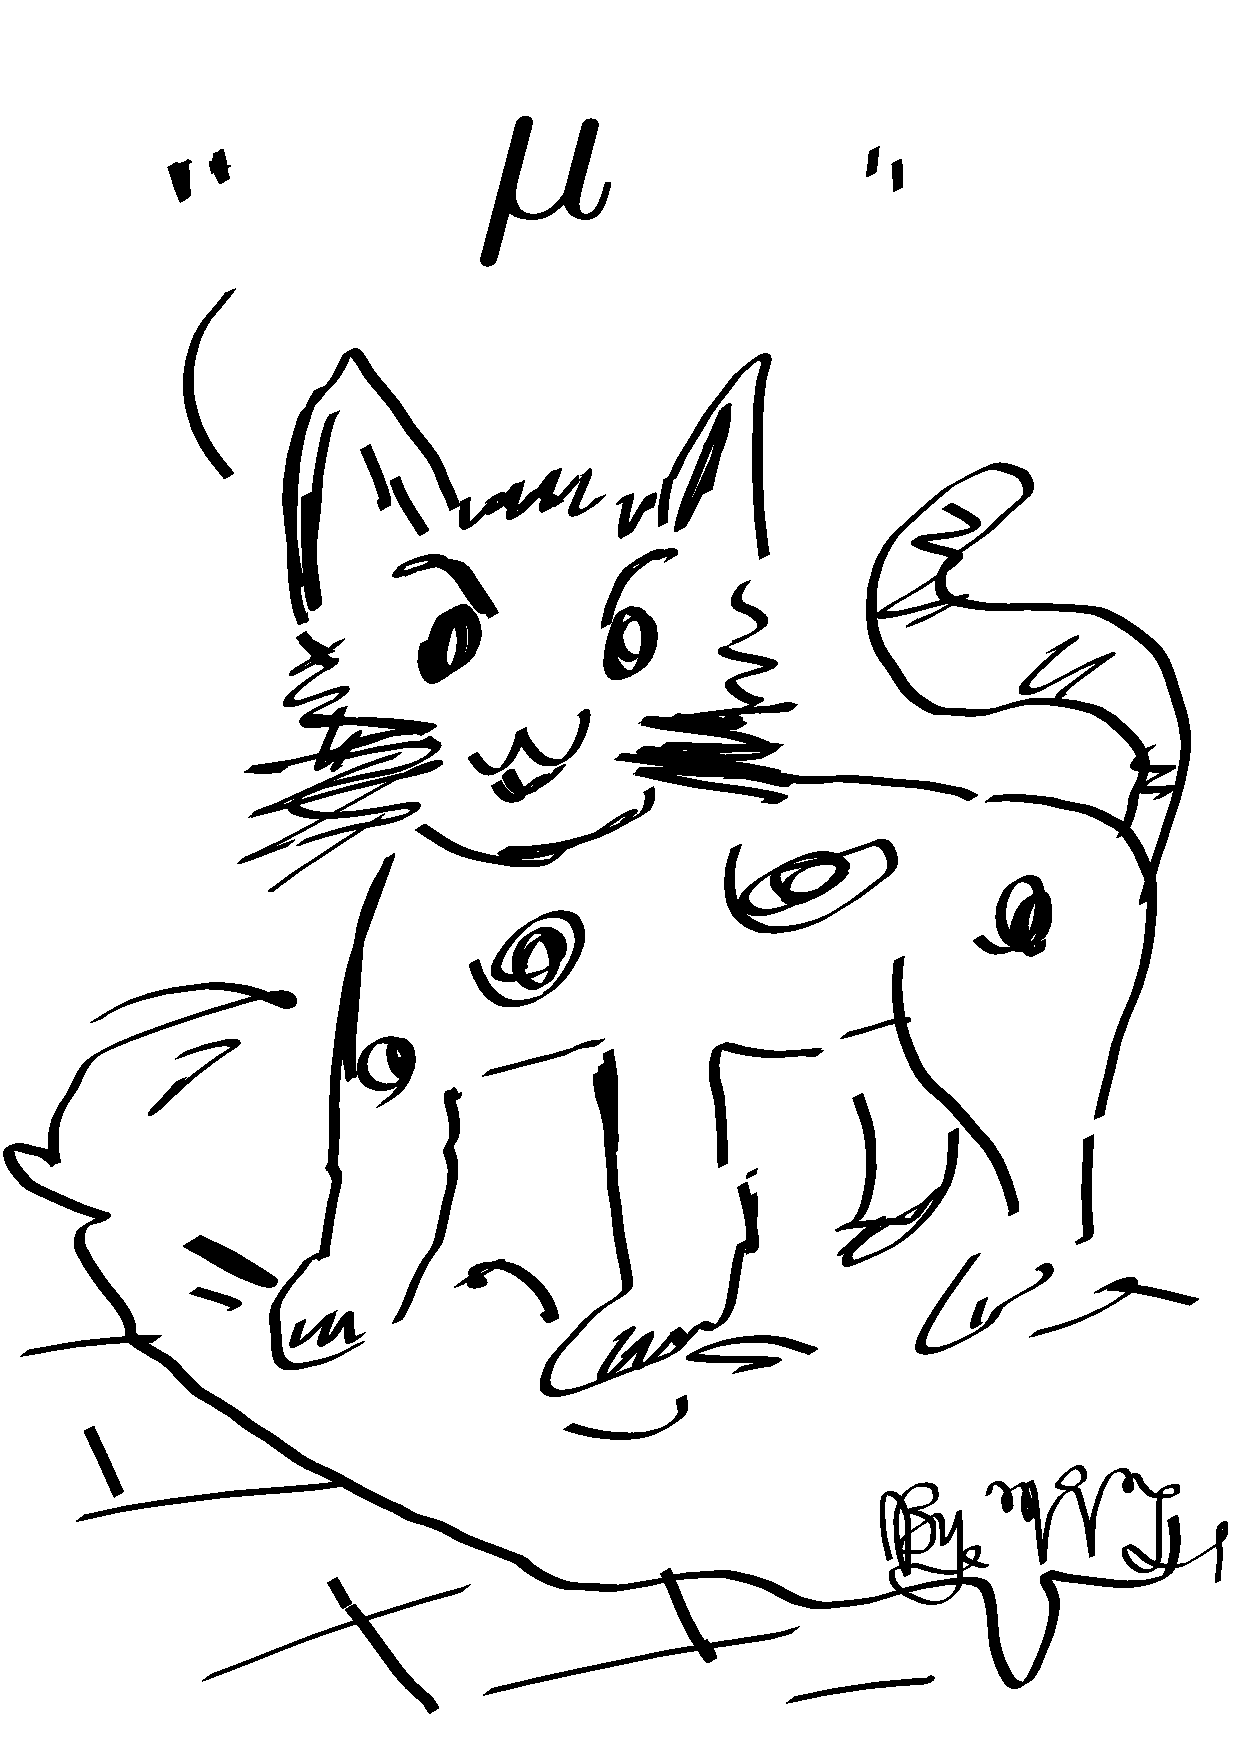
\includegraphics[width=8cm]{mucat.pdf}
  \caption{\textsl{"The $\mu$ cat"}, by Wang}
  \label{fig:cat_wang}
\end{figure}

\begin{figure}
	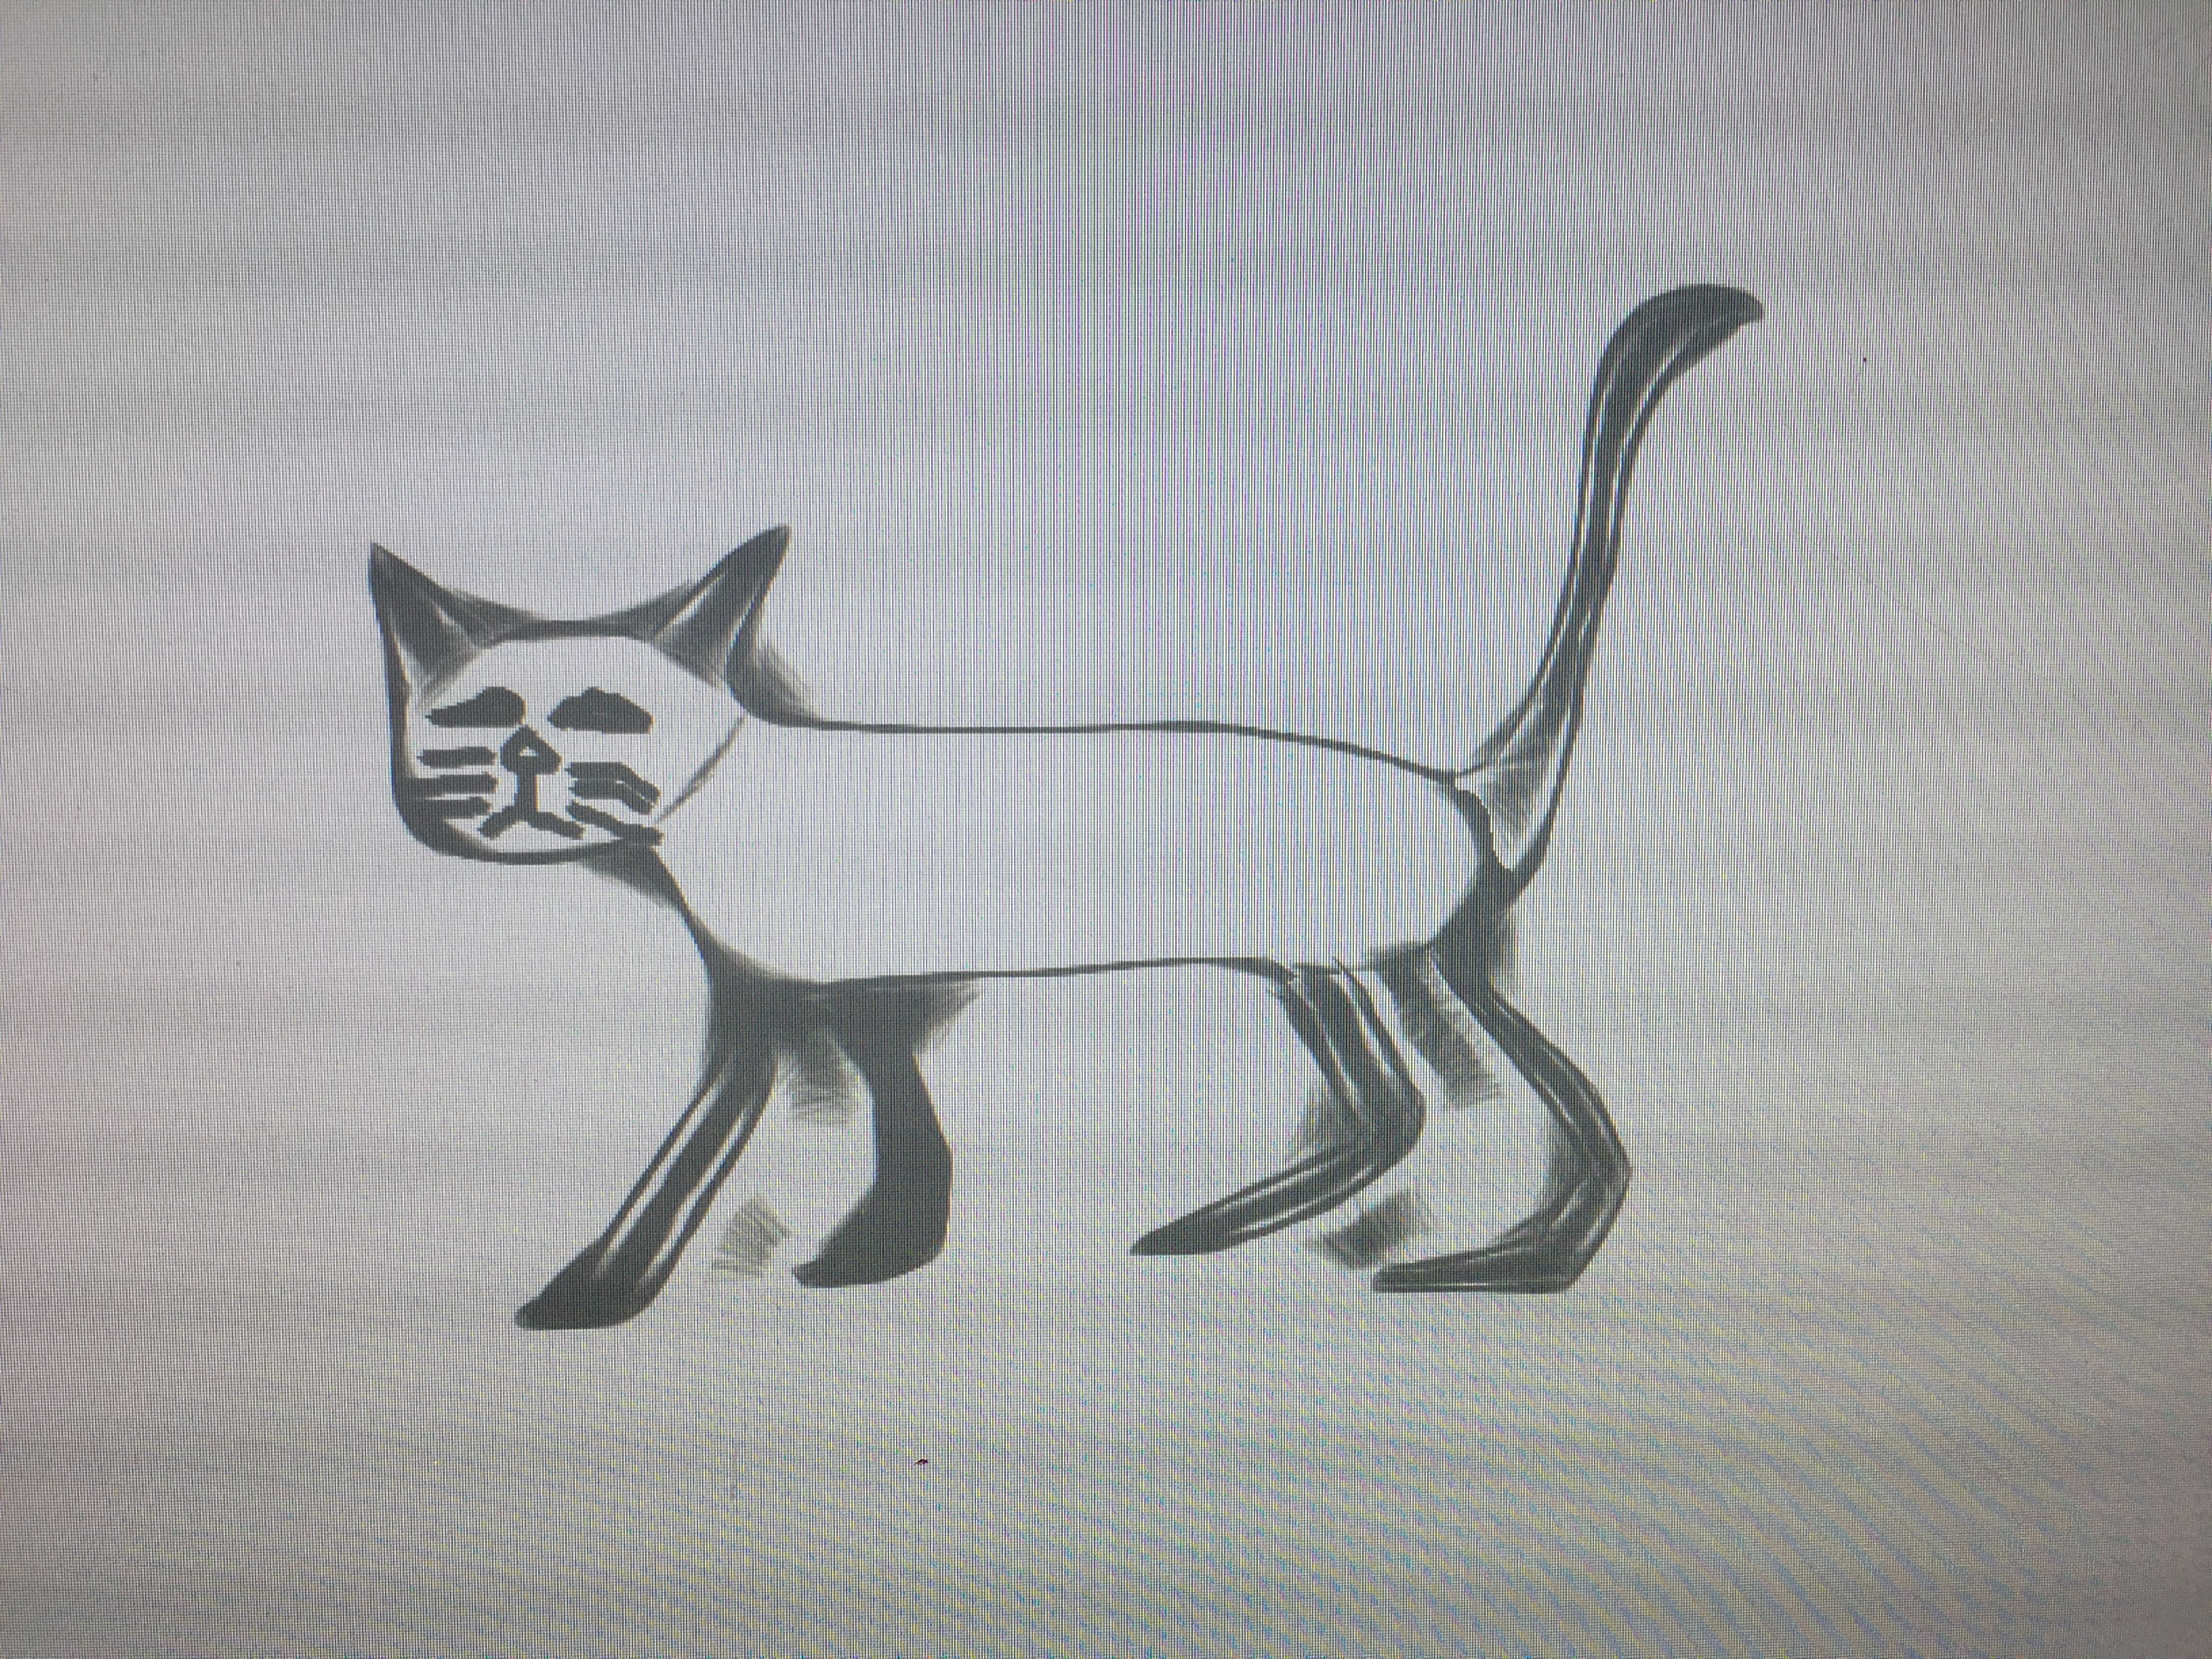
\includegraphics[width=8cm]{catsketch.pdf}
  \caption{Frazer's Cat Sketch}
  \label{fig:catsketch}
\end{figure}

\begin{figure}
	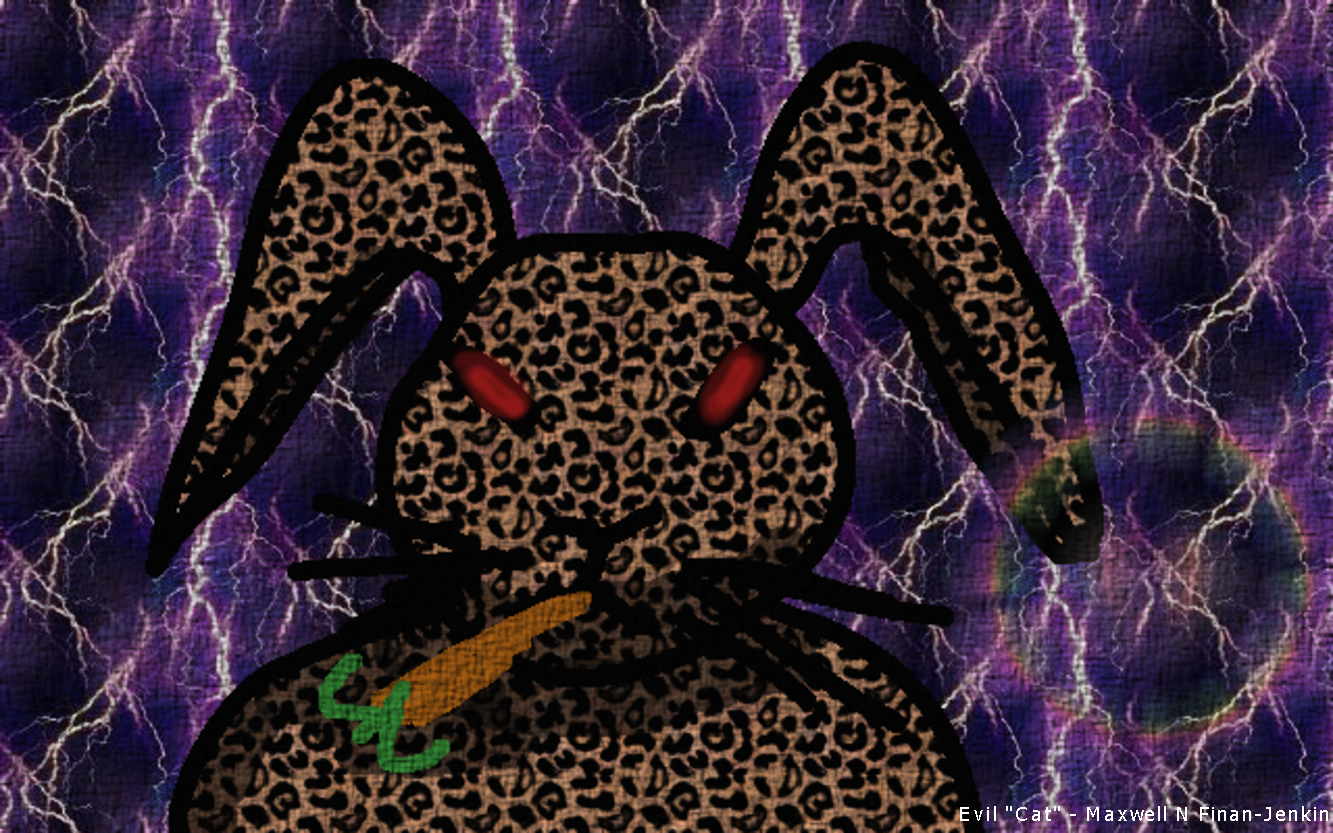
\includegraphics[width=8cm]{catto.pdf}
  \caption{An evil 'Cat' that Maxwell drew}
  \label{fig:catto}
\end{figure}



\begin{figure}
	\includegraphics[width=8cm]{cat742afer228.pdf}
  \caption{A cat that Alex drew.}
  \label{fig:cat_alex}
\end{figure}


\begin{figure}[H]
	\centering
	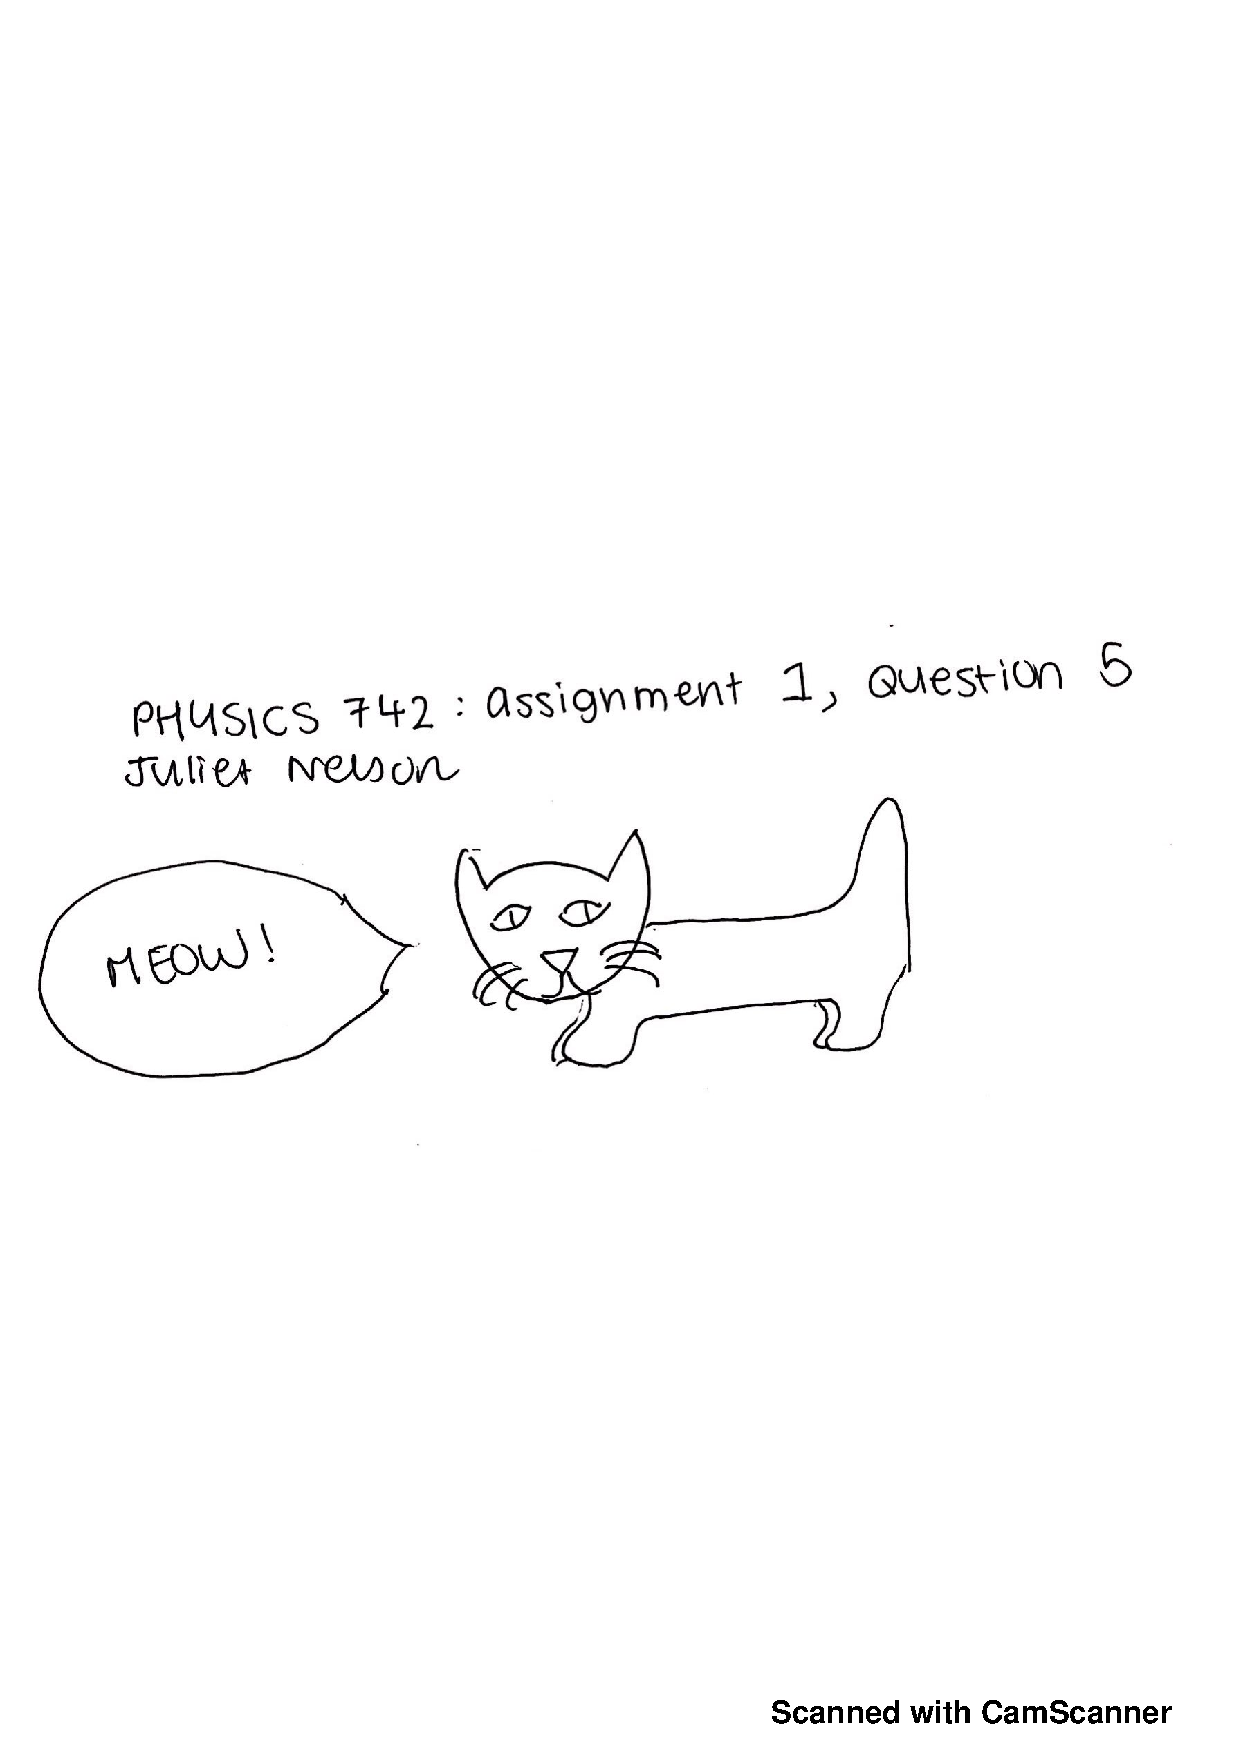
\includegraphics[width=8cm]{catjuliet.pdf}
	\caption{A cat that Juliet drew.}
	\label{fig:cat2}
\end{figure}



\begin{figure}
	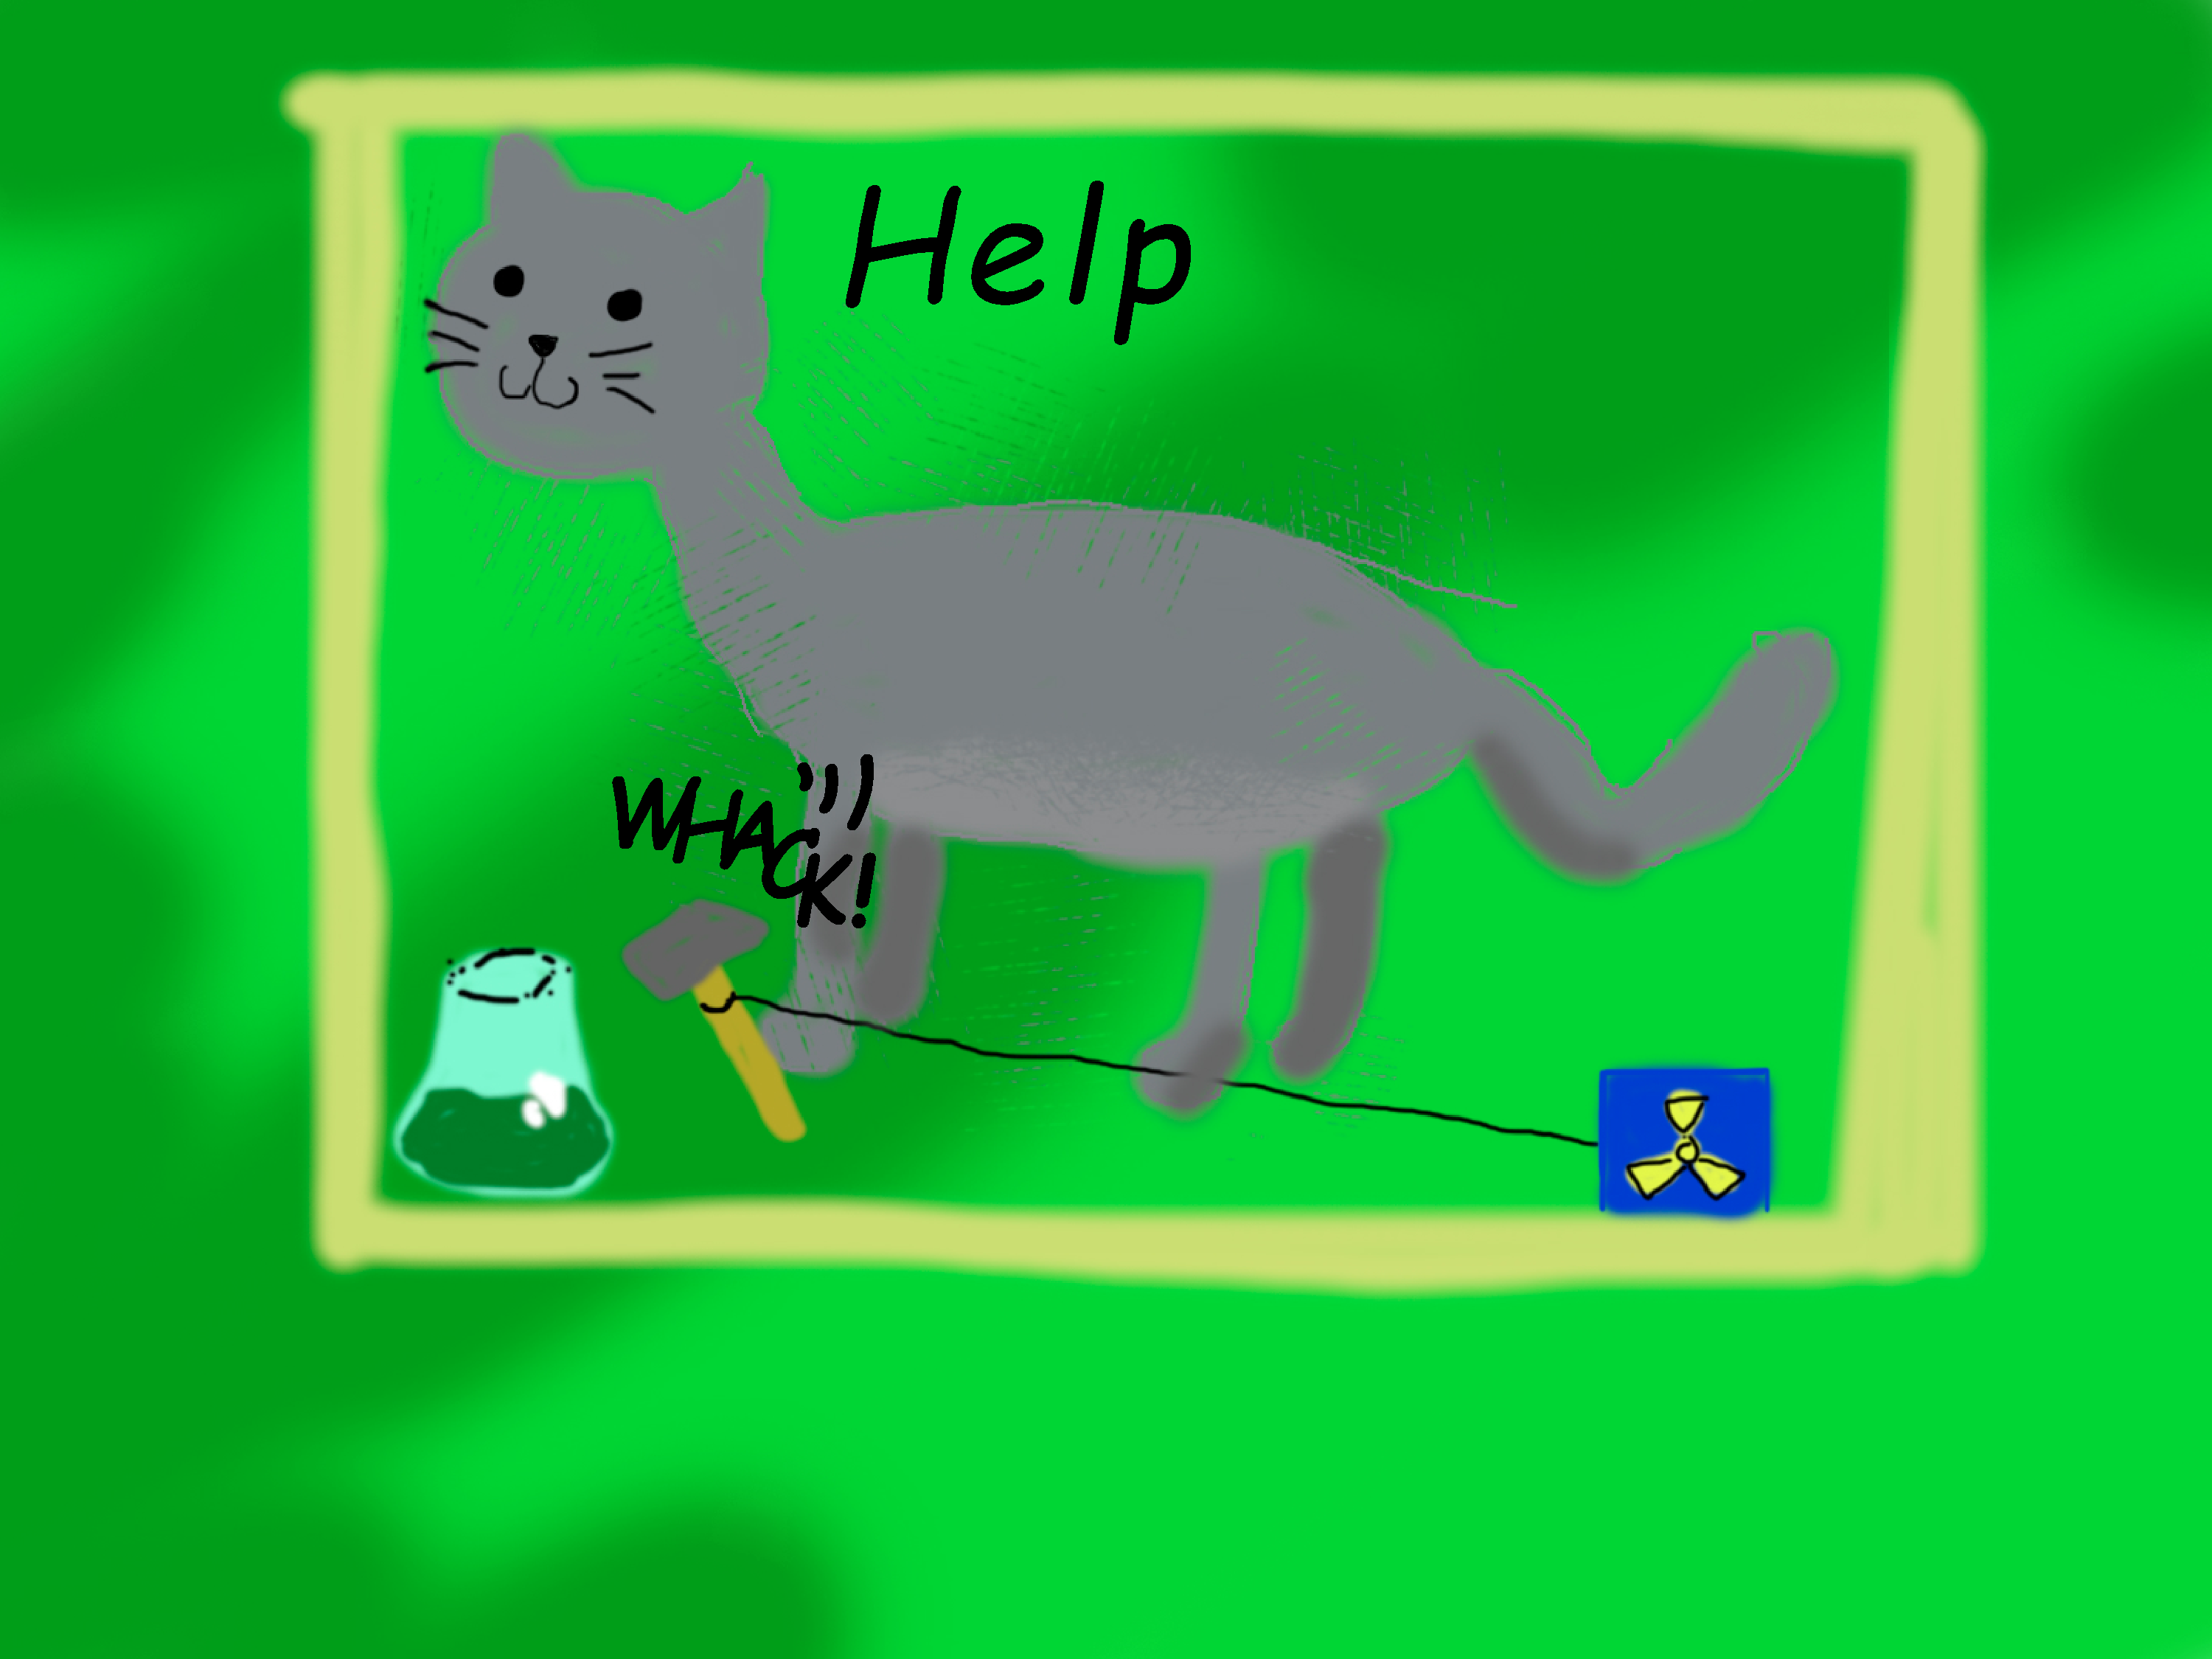
\includegraphics[width=8cm]{cat-gleb.pdf}
  \caption{let's be honest: it's probably dead. Gleb }
  \label{fig:cat_gleb}
\end{figure}



\begin{figure}
	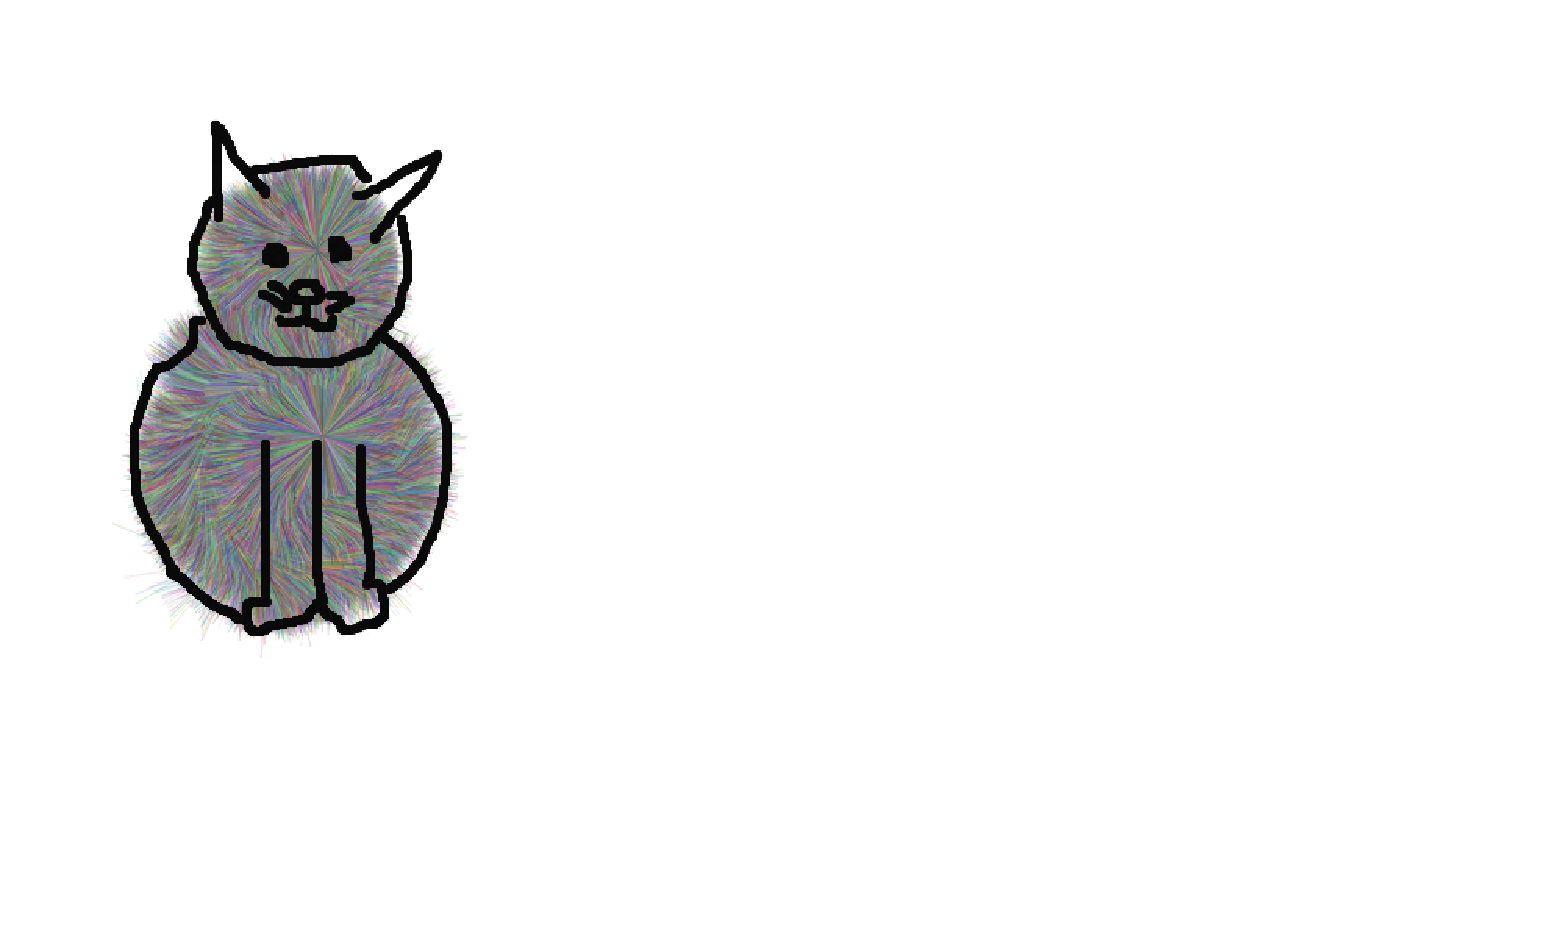
\includegraphics[width=8cm]{Cat742afer228.pdf}
  \caption{A cat that Kamrun drew.}
  \label{Cat draw by Kamrun}
\end{figure}




\begin{figure} \centering
    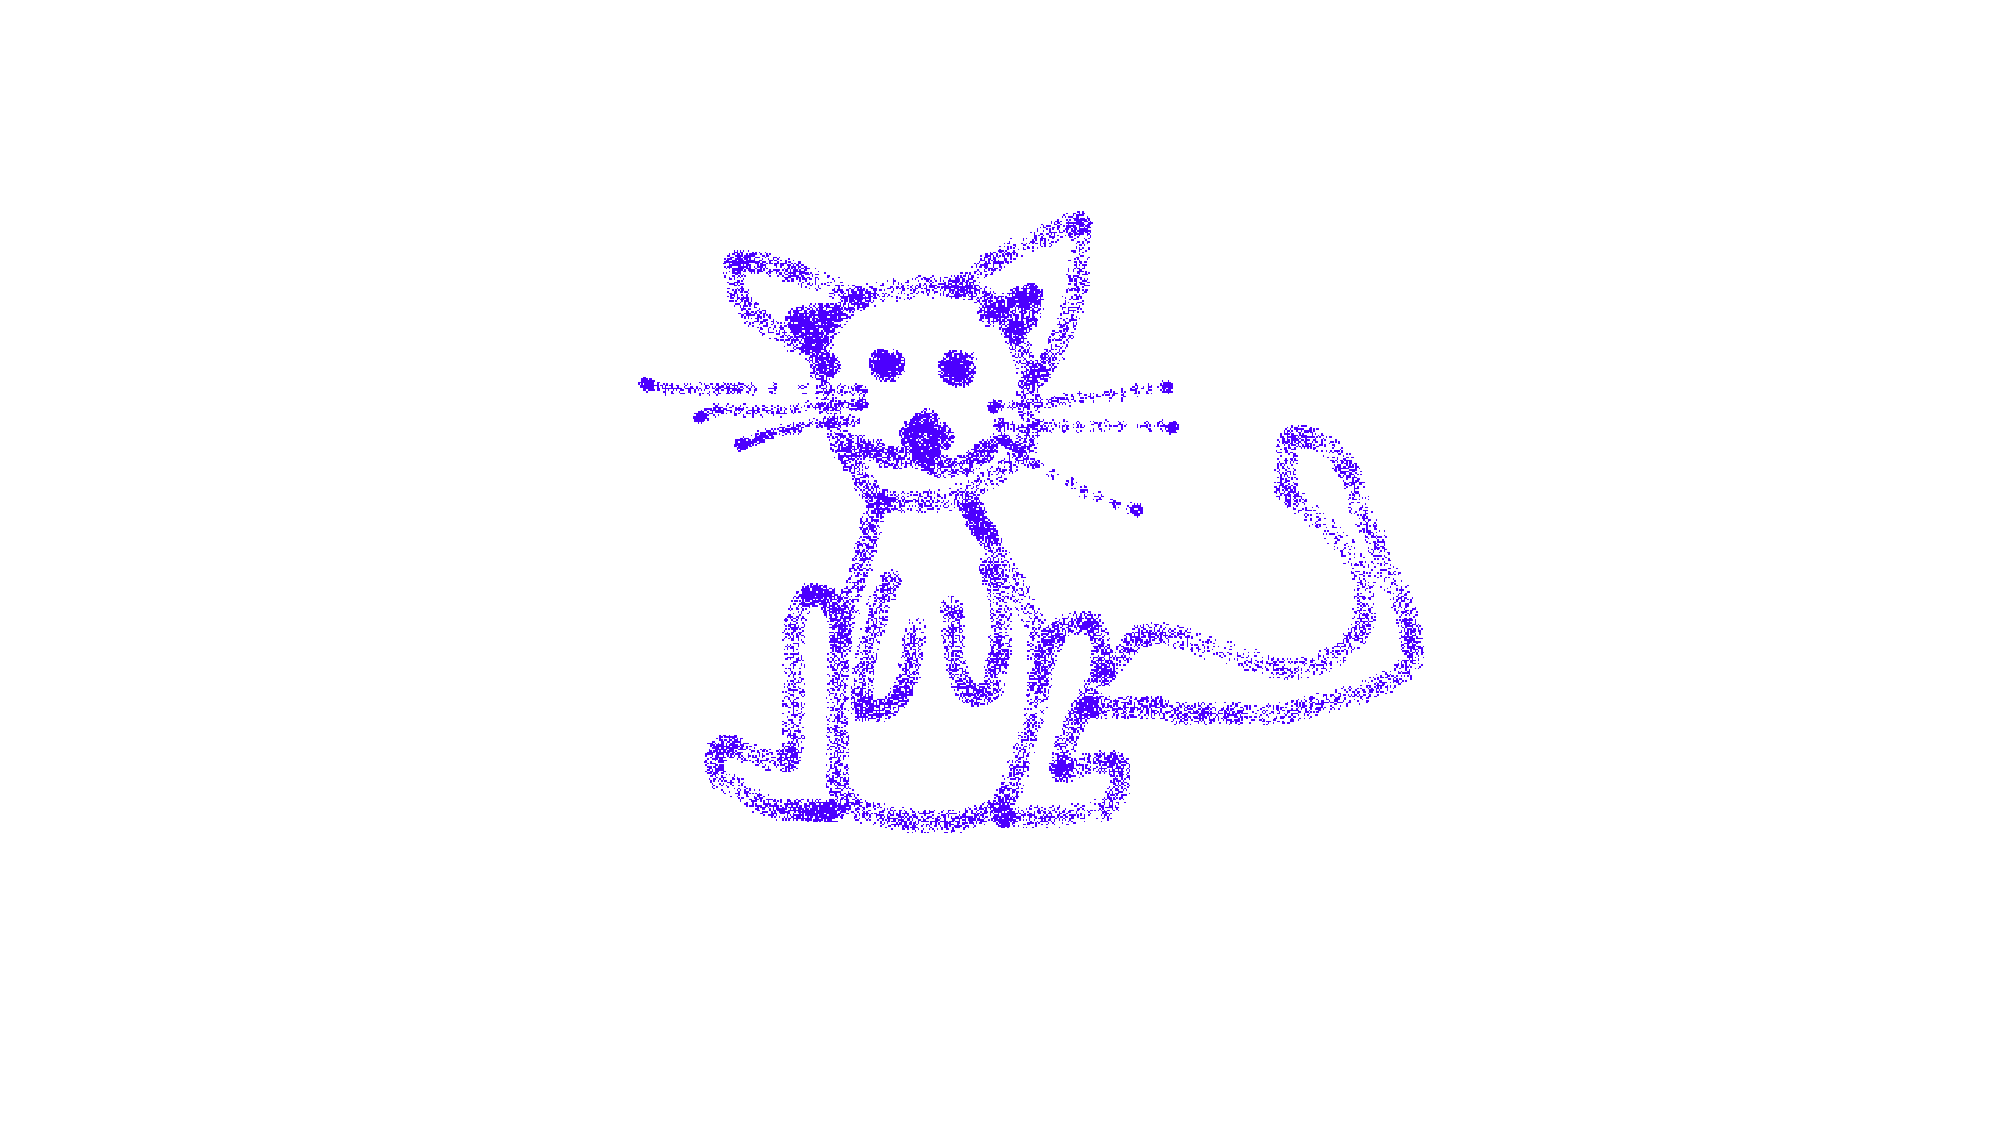
\includegraphics[width=8cm]{kat.pdf}
    \caption{\emph{``Kat"}, by Jasmine}
    \label{kat}
\end{figure}


\begin{figure}\centering
  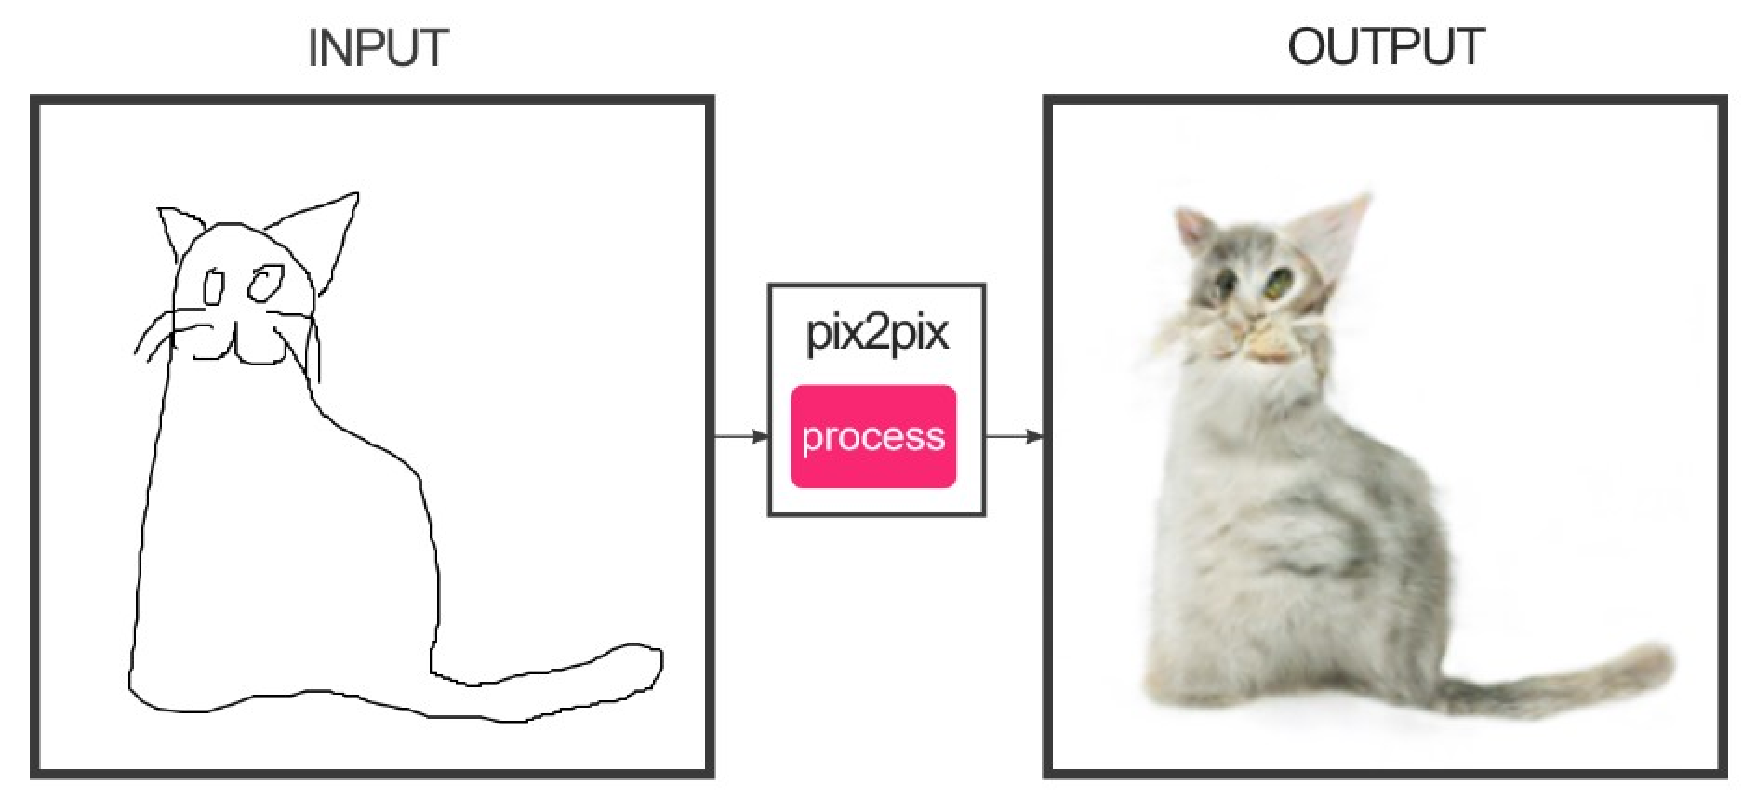
\includegraphics[width=8cm]{cat-fadiwassaf.pdf}
  \caption{I needed some help. Courtesy of edges2cats on https://affinelayer.com/pixsrv. - Fadi}
  \label{cat-fadi}
\end{figure}



\begin{figure}
	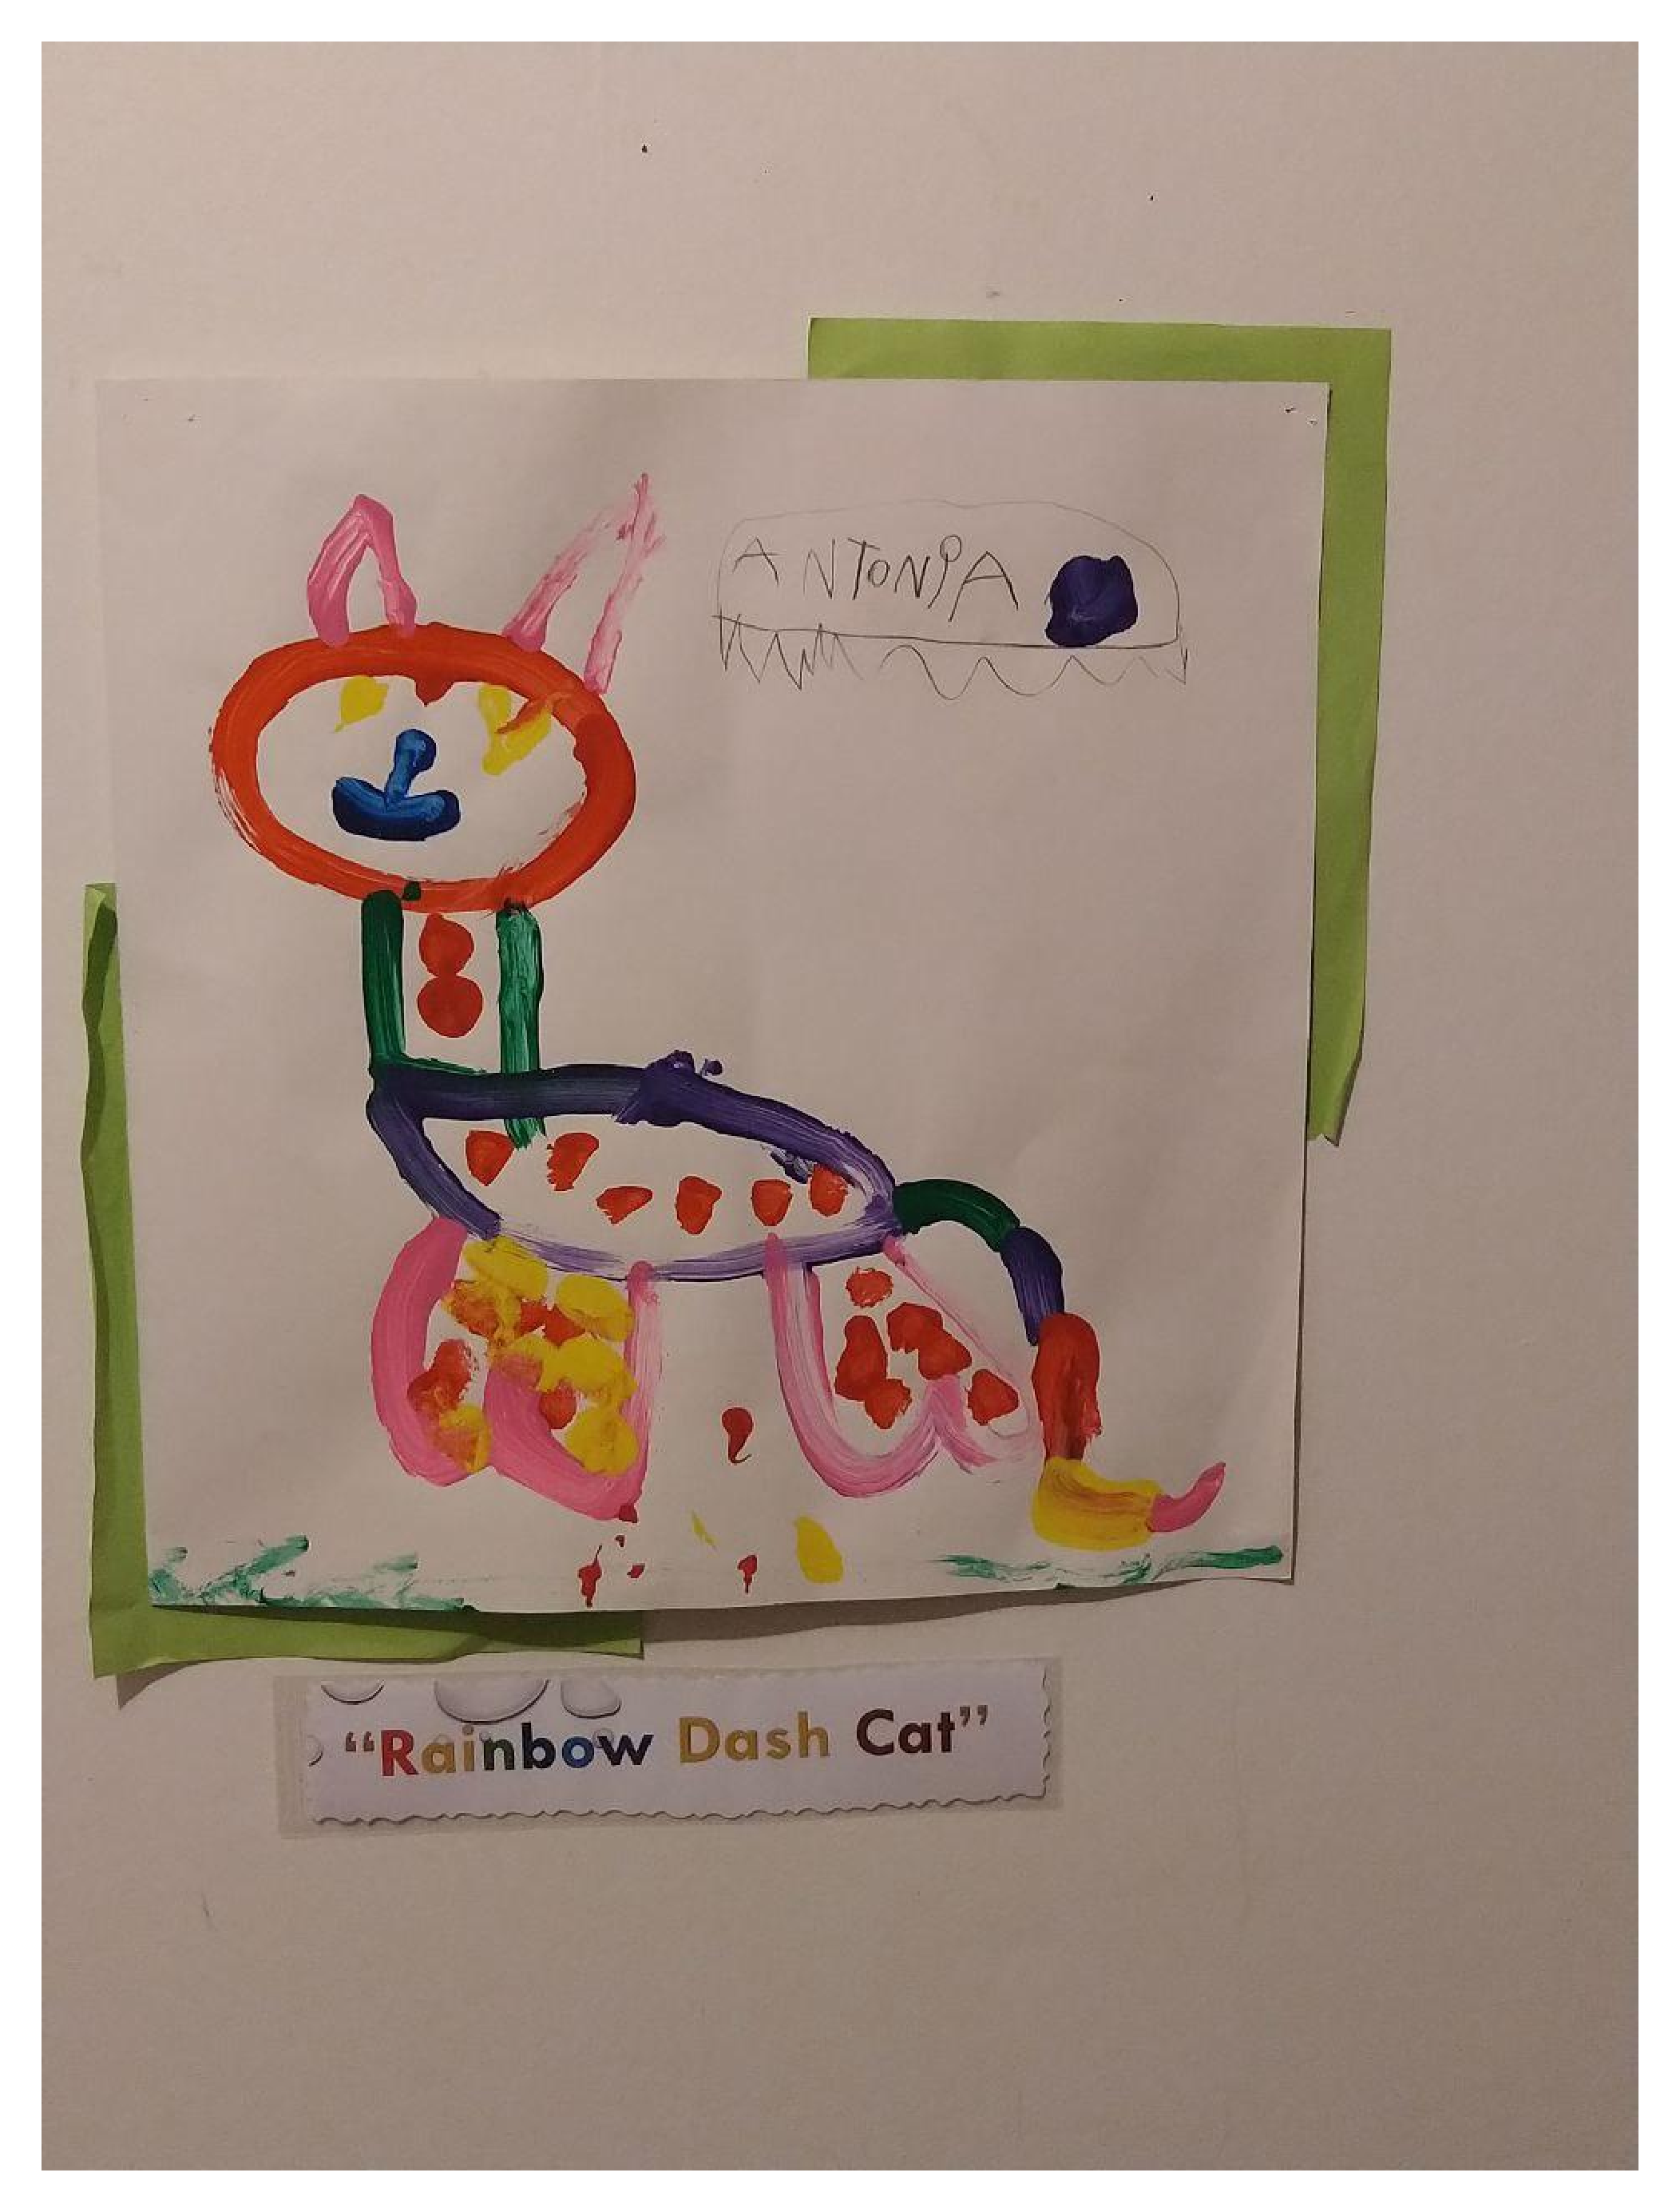
\includegraphics[width=8cm]{GrayCatPic.pdf}
  \caption{Gray's Cat Sketch}
  \label{Rainbow Dash Cat}
\end{figure}


\end{centering}

\clearpage

\section{Notes on Liouville's theorem from assignment one}
%\input{dionA1liouville.tex}

\subsection{Fadi Wassaf}

\noindent Let $\Gamma$ be the set of points in your phase space that satisfy the equations of motion for your system. Liouville's theorem states that for an initial $\Gamma^1$ and some $\Gamma^2$ at a later point in time, then $|\Gamma^1| = |\Gamma^2|$. In other words, phase space volumes are conserved through time evolution for a Hamiltonian system. An alternative description may be that $\rho$, the local density (or probability density) of microstates, will stay constant along the trajectories through phase space.\\

\noindent If this wasn't true, then we might not have the ability to work with microstates the way we do now. For example, if the volume (which corresponds to the number of microstates) increased with time evolution, then we'd suddenly new microstates magically coming into existence over time. Given that we have defined entropy as $S=k\ln |\Gamma|$, this would suggest that the entropy of the system would keep increasing and not stay to an equilibrium point.\\

\noindent Liouville's theorem is useful when talking about systems in equilibrium. Given the restriction that\\ $\partial \rho / \partial t = 0$, we know that all ensemble averages will not depend on time. An ensemble where this is the case is stationary. We can then represent a system at equilibrium by a stationary ensemble since the probability distribution is independent of time.



\end{document}
